\documentclass{book}
\usepackage{ragged2e}

\usepackage{graphicx} % Required for inserting images
\usepackage[spanish, english]{babel}
\usepackage[hidelinks]{hyperref}
%----------------------------------------
% BIBLATEX + BIBER
\usepackage[backend=biber,style=alphabetic,sorting=nyt,language=spanish]{biblatex}
\addbibresource{bibliografia.bib}
%----------------------------------------

\usepackage{makecell}
\usepackage[numbered,framed]{listings}
\usepackage{color} % red, green, blue, yellow, cyan, magenta, black, white
\usepackage{enumitem}
\usepackage{lmodern}
\usepackage{microtype} 
\usepackage{array}
\usepackage{float}
\usepackage{tabularx}
\usepackage{siunitx}
\usepackage{booktabs}
\usepackage{footnote}          % <— nuevo
\usepackage{siunitx}
\usepackage{inputenc}
\usepackage{threeparttable}
\usepackage{tikz}       % Diagrama en capas (cubo)
\usepackage{footmisc}   % Mejor gestión de notas a pie de página (opcional)
\usepackage{adjustbox}
\definecolor{mylilas}{RGB}{170,55,241}
\definecolor{backcolour}{rgb}{0.92,0.95,0.95}

\usepackage[printonlyused]{acronym}

\usepackage{longtable}
\usepackage{geometry}
\usepackage{lipsum}

\usepackage{listings}
\usepackage{xcolor}
\lstdefinestyle{custom}{
    backgroundcolor=\color{black!5},           % Fondo más sutil (gris muy claro)
    basicstyle=\ttfamily\footnotesize,         % Fuente monoespaciada más pequeña y profesional
    keywordstyle=\color{blue!70!black},        % Palabras clave en azul oscuro
    stringstyle=\color{orange!80!black},       % Cadenas en naranja suave
    commentstyle=\color{gray!50},              % Comentarios en gris claro
    numberstyle=\tiny\color{gray!40},          % Números de línea discretos
    numbers=left,                              % Números a la izquierda
    numbersep=10pt,                            % Espaciado entre números y código
    breaklines=true,                           % Romper líneas largas
    breakatwhitespace=true,                    % Romper solo en espacios
    frame=tb,                                  % Marco solo arriba y abajo (más elegante)
    framesep=5pt,                              % Espaciado interno del marco
    captionpos=b,                              % Título debajo
    showstringspaces=false,                    % No mostrar espacios en cadenas
    tabsize=4,                                 % Tamaño de tabulación
    escapeinside={(*@}{@*)},                   % Permitir escapar a LaTeX dentro del código
    morekeywords={app, def, return, send, register_blueprint, SocketIO} % Palabras clave adicionales
}


\newcolumntype{L}[1]{%
  >{\setlength\parindent{1em}% sangría primera línea
    \raggedright\arraybackslash}%
  p{#1}%
}

\AtBeginDocument{\justifying}
\begin{document}

\frontmatter


% Configurando la numeración arábiga desde el inicio
\pagenumbering{arabic}

% Creando la portada
\begin{titlepage}
    \centering
    {\includegraphics[width=0.9\textwidth]{Imagenes/Universidad-de-Valladolid.png}}\par
    {\bfseries\Large Escuela Técnica Superior de Ingenieros de Telecomunicación\par}
    \vspace{0.5cm}
    {\bfseries\itshape\Large Trabajo de Fin de Grado \par}
    \vspace{0.5cm}
    {\scshape Grado en Ingeniería de Tecnologías de Telecomunicación \par}
    \vspace{0.5cm}
    {\bfseries\scshape\Large \textit{Request To Pay} frente a la domiciliación bancaria: propuesta de mejora e implementación de un prototipo \par}
    \vspace{1.5cm}
    { Autor: \\}
    { Alonso Sandoval Martínez }\\
    \vspace{0.5cm}
    { Tutor:\\}
    { Federico Simmross Wattenberg }\\
    \vspace{1.5cm} {Valladolid, junio 2025 \par}
\end{titlepage}

% Configurando el idioma
\selectlanguage{spanish}  

% Añadiendo los agradecimientos desde un archivo externo
\newpage
\phantomsection
\addcontentsline{toc}{section}{Agradecimientos}

\thispagestyle{empty}       % sin cabecera ni número de página

\vspace*{\fill}             % empuja el bloque hacia el centro vertical
\begin{center}
\chapter*{Agradecimientos}

Agradezco, en primer lugar, la orientación y el seguimiento de mi tutor,  
cuya experiencia ha sido decisiva para completar este trabajo.

Extiendo mi gratitud a mi familia por su respaldo constante y a mis amigos  
por el apoyo práctico y la paciencia mostrada durante el desarrollo del proyecto.

Su ayuda conjunta ha permitido que este trabajo llegue a buen término.
\end{center}
\vspace*{\fill}             % completa el centrado vertical


% Añadiendo el resumen en español
\newpage
\phantomsection
\addcontentsline{toc}{section}{Resumen}

\thispagestyle{empty}
\selectlanguage{spanish}

\chapter*{Resumen}
En España, la domiciliación bancaria, regulada bajo el esquema \textit{SEPA\cite{ecb_sepa} Direct Debit} (SDD), es el método predominante para los cobros recurrentes. Este sistema permite a los acreedores realizar cargos automáticos en las cuentas de los deudores con una autorización previa. Sin embargo, presenta varias limitaciones que dificultan su adaptación a la economía digital actual.

Frente a estas limitaciones, surge el esquema \textit{SEPA} Request-to-Pay} (SRTP) como una alternativa moderna. El SRTP permite a los beneficiarios enviar solicitudes de pago digitales a los pagadores, quienes pueden aceptarlas, rechazarlas o aplazarlas en tiempo real, utilizando la infraestructura de pagos instantáneos \textit{SEPA (SCT Inst)}.

Este Trabajo de Fin de Grado tiene como objetivo explicar y demostrar el funcionamiento del SRTP como solución a las carencias del SDD. Para ello, se propone el diseño e implementación de un prototipo que simula el ciclo completo de una petición de pago: creación, presentación, decisión, ejecución y cierre. El prototipo se basa en una API desarrollada con un servidor web Flask, que gestiona las interacciones entre los actores del ecosistema SRTP (beneficiarios, pagadores y proveedores de servicios de pago) mediante una arquitectura orientada a eventos y una interfaz web en tiempo real.

\newpage

\selectlanguage{english}
\chapter*{Abstract}
In Spain, bank direct debit, regulated under the \textit{SEPA Direct Debit} (SDD) scheme~\cite{ecb_sepa}, is the predominant method for the collection of recurring payments. This arrangement allows creditors to initiate automatic debits from debtors' accounts once prior authorisation has been granted. Nevertheless, it exhibits several limitations that hinder its adaptation to the current digital economy.

To overcome these limitations, the \textit{SEPA Request-to-Pay} (SRTP) scheme has emerged as a modern alternative. SRTP enables beneficiaries to send digital payment requests to payers, who can accept, reject or defer them in real time by using the \textit{SEPA Instant Credit Transfer} (SCT Inst) infrastructure.

This bachelor thesis aims to explain and demonstrate how SRTP remedies the shortcomings of SDD. With this purpose, it proposes the design and implementation of a prototype that simulates the entire life cycle of a payment request: creation, presentation, decision, execution and closure. The prototype is based on an API implemented with a Flask web server, which manages the interactions among the actors within the SRTP ecosystem (beneficiaries, payers and payment service providers) by means of an event driven architecture and a real time web interface.


% Añadiendo el índice justo después de la portada
\newpage
\tableofcontents

\newpage
\phantomsection % Añade un destino para el hipervínculo
\chapter*{Lista de acrónimos}
\label{sec:Lista de acrónimos}
\addcontentsline{toc}{section}{Lista de acrónimos} % Añade al índice con el destino correcto
\begin{acronym}[SRTP]
\begin{enumerate}
  \item API – Application Programming Interface
  \item CDN – Content Delivery Network
  \item CSS3 – Cascading Style Sheets 3
  \item EBA – Euro Banking Association
  \item EDS – Electronic Data Submission
  \item EDS-Dir – EPC Directory Service
  \item EPC – European Payments Council
  \item ERPB – Euro Retail Payments Board
  \item ES6 – ECMAScript 6
  \item HTML5 – HyperText Markup Language 5
  \item HTTP – Hypertext Transfer Protocol
  \item IBAN – International Bank Account Number
  \item ISO20022 – International Organization for Standardization 20022
  \item JSON – JavaScript Object Notation
  \item NFC – Near Field Communication
  \item ORM – Object-Relational Mapping
  \item POS – Point of Sale
  \item PSD2 – Payment Services Directive 2
  \item PSP – Payment Service Provider
  \item QR – Quick Response
  \item RTP – Request-to-Pay
  \item SCA – Strong Customer Authentication
  \item SCT – SEPA Credit Transfer
  \item SCT Inst – SEPA Instant Credit Transfer
  \item SEPA – Single Euro Payments Area
  \item SDD – SEPA Direct Debit
  \item SRTP – SEPA Request-to-Pay
  \item TCP – Transmission Control Protocol
  \item TFG – Trabajo de Fin de Grado
  \item TIPS – TARGET Instant Payment Settlement
  \item TPV – Terminal Punto de Venta
  \item WSGI – Web Server Gateway Interface
\end{enumerate}
\end{acronym}

% Volviendo al español para el resto del documento
\selectlanguage{spanish} 

\mainmatter

% Comenzando el cuerpo principal (numeración ya es arábiga)
\newpage



\chapter{Introducción}
\label{sec:Introduccion}

Para comprender el entorno actual de los pagos en Europa, conviene arrancar por la \emph{Single Euro Payments Area} (SEPA): un espacio comunitario en el que todos los pagos en euros se rigen por los mismos estándares técnicos y normas operativas, de modo que enviar dinero de un país a otro resulta tan ágil y claro como una transferencia nacional\cite{ecb_sepa}. SEPA estableció protocolos de mensajería comunes, armonizó los plazos de liquidación y fijó reglas uniformes de protección al usuario, creando la base sobre la que se despliegan hoy los servicios de pago más innovadores.

En los últimos diez años, la digitalización de los servicios financieros ha cambiado por completo cómo particulares y empresas gestionan sus transacciones dentro de ese marco SEPA. Las transferencias instantáneas, las API abiertas de los bancos y el auge del comercio electrónico han disparado la demanda de procesos de cobro que sean sencillos, transparentes y en tiempo real. No obstante, los instrumentos de pago tradicionales (tarjetas, transferencias convencionales o domiciliaciones) nacieron en un contexto muy distinto y todavía arrastran limitaciones que penalizan tanto la experiencia de usuario como la eficiencia operativa.

Aquí es donde entra en juego \emph{Request-to-Pay} (RTP). Este servicio de mensajería permite al beneficiario enviar al pagador una solicitud de pago digital estructurada, con todos los detalles (importe, concepto, vencimiento), y recibir en segundos una respuesta (aceptación, rechazo o aplazamiento) antes de iniciar el movimiento de fondos. RTP no sustituye los métodos de pago existentes, sino que actúa como una capa de orquestación sobre la infraestructura SEPA (y, en especial, los pagos inmediatos) y los canales de banca online, facilitando la conciliación, reduciendo la fricción en el cobro y modernizando la experiencia tanto para empresas como para consumidores.

\section{Motivación}
\label{subsec:Motivacion}

La domiciliación bancaria, regulada por el esquema \textit{SEPA Direct Debit} (\textbf{SDD})\cite{epc_sdd_2025} (instrumento paneuropeo de cargo en cuenta regulado por el \emph{European Payments Council} (EPC)) desde 2014, sigue siendo el método principal para cobros recurrentes en España. No obstante, su estructura, pensada para un entorno de procesos \emph{offline} genera hoy inconvenientes que chocan con las demandas de inmediatez, seguridad y experiencia de usuario fluida que caracterizan la economía digital actual. Así se detectan una serie de ineficiencias, que se describen en la sección \ref{subsec:ineficiencias}, y una oportunidad de introducir un nuevo método de pago que solvente dichas ineficiencias, el cual se presenta en la sección \ref{subsec:oportunidadRTP}.

\subsection{Ineficiencias operativas detectadas}
\label{subsec:ineficiencias}

Tras analizar la operativa SDD nacional se han identificado una serie de ineficiencias que afectan tanto a los usuarios como a las entidades participantes en el proceso de pago resumidas en los siguientes \textbf{5} puntos:
\begin{enumerate}[label=\textbf{\arabic*.}, leftmargin=0.75cm]
      \item \textbf{Modelo offline y necesidad de mandato físico}\\
            El proceso de pago mediante el esquema SDD opera bajo un modelo offline, lo que implica una ausencia total de interacción en tiempo real entre las partes involucradas. Para iniciar el cobro, el deudor debe firmar y enviar un \textbf{mandato SEPA} en formato físico. Este mandato es un documento mediante el cual el deudor autoriza al acreedor a realizar cobros automáticos a través de la domiciliación bancaria. El documento debe ser conservado por el acreedor durante toda la duración del contrato y hasta 14 meses después de la última transacción realizada. Aunque la digitalización ha avanzado en muchos ámbitos, aún no existe un estándar único y interoperable para los \textit{\textbf{eMandates}}, que son la versión electrónica de los mandatos SEPA que permitem autorizar cobros de manera digital, lo que lleva a que cada entidad bancaria implemente su propio sistema. Esta falta de uniformidad genera inconsistencias y dificulta la estandarización del proceso.\\
            \textbf{Consecuencias}:
      \begin{itemize}
            \item Fricciones significativas en los procesos de venta digital, ya que los usuarios deben completar pasos adicionales que rompen con la inmediatez esperada en el comercio electrónico actual.
            \item Costes operativos considerables asociados a la gestión administrativa, como el archivado, las auditorías y el mantenimiento de los mandatos físicos.
            \item Riesgos legales y financieros en caso de disputa, como devoluciones costosas o conflictos prolongados con los deudores, debido a la ausencia de un mandato válido.
      \end{itemize}

  \item \textbf{Derecho a devolución prolongado}\\
        El esquema SDD otorga al deudor un derecho a devolución excepcionalmente amplio, lo que genera incertidumbre en la gestión de los ingresos por parte de los acreedores. En el caso de un \emph{cobro autorizado}, el deudor puede solicitar la devolución del importe sin necesidad de justificar su decisión durante un periodo de \textbf{ocho semanas}, bajo la política conocida como \emph{“no-questions-asked”}. Por otro lado, si el cobro se clasifica como \emph{no autorizado} (por ejemplo, si el banco emisor no puede probar la existencia de un mandato válido), el plazo para reclamar se extiende hasta \textbf{trece meses}.
        
        \textbf{Consecuencias}:
        \begin{itemize}
          \item Notable inseguridad para los acreedores, quienes deben mantener reservas de liquidez y provisiones contables para cubrir posibles devoluciones tardías.
          \item Facilitación de prácticas como el \emph{friendly fraud}\footnote{El \emph{friendly fraud} ocurre cuando un usuario consume un bien o servicio y, posteriormente, solicita una devolución sin justificación, aprovechando las políticas de devolución laxas.}, donde los deudores reclaman reembolsos injustificados tras haber recibido el producto o servicio.
          \item Impacto directo en la rentabilidad de las empresas debido a las devoluciones inesperadas.
        \end{itemize}

  \item \textbf{Ciclos de cobro lentos}\\
        Los tiempos de procesamiento en el esquema SDD son significativamente prolongados, lo que compromete tanto la eficiencia operativa como la experiencia del usuario. En el esquema \textsc{Core} \cite{epc016}, el acreedor debe enviar la orden de cobro al banco con una antelación de \textbf{D-5 días} para la primera domiciliación y de \textbf{D-2 días} para las domiciliaciones recurrentes. A esto se suman \textbf{dos días adicionales} para la liquidación interbancaria. En total, el proceso puede demorar entre seis y ocho días naturales desde que se solicita el cobro hasta que se confirma el abono, un plazo incompatible con las expectativas de inmediatez en la venta de bienes o servicios digitales.
        
        \textbf{Consecuencias}:
        \begin{itemize}
          \item Afectación en la planificación financiera de las empresas, ya que los ingresos no están disponibles de manera inmediata, generando una tesorería imprevisible.
          \item Riesgo de prestar servicios o entregar productos sin la certeza de que el pago se completará con éxito.
          \item Pérdidas económicas significativas debido a la falta de confirmación inmediata del pago.
        \end{itemize}

  \item \textbf{Costes y complejidad de las R-transactions}\\
        Las \textbf{R-transactions}, que son transacciones de rechazo, devolución o reembolso asociadas a pagos fallidos o no autorizados, representan una fuente notable de complicaciones y costes adicionales. Estas transacciones se clasifican mediante diversos códigos, cada uno asociado a un flujo y reglas específicas, lo que dificulta su gestión y seguimiento. Los acreedores deben dedicar recursos a identificar las causas de cada R-transaction y aplicar las medidas correctivas correspondientes, un proceso que frecuentemente requiere intervención manual debido a la falta de automatización.
        
        \textbf{Consecuencias}:
        \begin{itemize}
          \item Necesidad de equipos especializados en conciliación y recobro, incrementando los costes operativos.
          \item Reducción de la eficiencia general del sistema debido a la complejidad de los procesos.
          \item Posibilidad de errores o retrasos que afectan la productividad y la confianza en el esquema SDD.
        \end{itemize}

  \item \textbf{Ausencia de autorización fuerte}\\
        El esquema SDD se basa en un consentimiento previo otorgado mediante el mandato SEPA, pero no incorpora la \textbf{autorización fuerte del cliente (SCA)}, que es un requisito de seguridad que exige la verificación del usuario mediante al menos dos factores de autenticación \cite{EC_2018_RTS_SCA} en el momento de cada transacción. Una vez firmado el mandato, los cobros se ejecutan automáticamente sin que se solicite al deudor una autenticación adicional para cada operación.
        
        \textbf{Consecuencias}:
        \begin{itemize}
          \item Elevado riesgo de disputas por cargos no autorizados, lo que puede derivar en conflictos y devoluciones.
          \item Pérdida de una oportunidad clave para fortalecer la seguridad y la confianza en el proceso de cobro mediante métodos de autenticación modernos.
        \end{itemize}
\end{enumerate}

% Conclusión
\paragraph{En conclusión.} Estas ineficiencias tienen un gran impacto en la operativa y la competitividad de las empresas y entidades financieras que lo utilizan y se traducen en:

\begin{itemize}[leftmargin=0.45cm]
  \item Una \textbf{estructura de costes elevada}, derivada de la alta frecuencia de devoluciones y la necesidad de personal especializado para gestionarlas, lo que incrementa los gastos operativos.
  \item \textbf{Liquidez incierta}, ya que los ingresos no se confirman de inmediato y pueden ser revertidos incluso meses después de haberse registrado, dificultando la gestión financiera.
  \item Un \textbf{freno al desarrollo de la economía digital}, puesto que el SDD no está diseñado para ofrecer experiencias de pago instantáneas y fluidas, como las que proporcionan métodos alternativos como las tarjetas de crédito, los monederos electrónicos o plataformas como Bizum.
\end{itemize}

\subsection{Oportunidad de un esquema RTP}
\label{subsec:oportunidadRTP}
El estándar \textit{SEPA RTP} (\textbf{SRTP}) aborda de manera efectiva las limitaciones técnicas y operativas del SDD, ofreciendo una laternativa más ágil y adaptada al entorno digital.

A continuación se describen las principales ventajas del SRTP frente al SDD:

\begin{enumerate}[label=\alph*)]
  \item \textbf{Autenticación reforzada y consentimiento digital inmediato}\\
      El SRTP reemplaza el mandato físico del SDD por una solicitud de pago que el deudor aprueba directamente desde su banca en línea o wallet digital mediante SCA. Este proceso genera una prueba eléctronica de consentimiento, firmada y resgistrada en el sistema del Payment Service Provider (PSP) del pagador, eliminando la dependencia de documentos en papel y simplificando la gestión de autorizaciones.

  \item \textbf{Irrevocabilidad y mitigación de fraude \emph{post-servicio}}\\
      Una vez aceptada la solicitd, el pago se ejecuta mediante SCT Inst, que es una transferencia inmediata SEPA con liquidación en menos de 10 s \cite{epc_sctinst_2025}. A diferencia del SDD que permite devoluciones automáticas en plazos amplios, el SRTP no admite reversiones sin causa justificada. Esto minimiza el riesgo de \textit{friendly fraud} y reduce la necesidad de provisiones por impagos.

  \item \textbf{Liquidez \emph{real-time} y conciliación automática}\\
      Con fondos disponibles en menos de 10 segundos, las empresas pueden gestionar su tesorería con mayor precisión. Además, el uso de identificadores únicos y referencias estructuradas según el estándar ISO 20022 \cite{iso20022_55005}, asegura que la información del pago se transmita íntegramente de extremo a extremo, permitiendo una conciliación automática y eliminando los retrasos y errores típicos del SDD.

  \item \textbf{Simplificación operativa}\\
      El SRTP elimina las R-transactions, la custodia de mandatos físicos y las tareas administrativas asociadas. El flujo se reduce a dos mensajes principales -solicitud y aceptación-, con la opción de una transferenciua instantánea, ofreciendo una trazabilidad clara y directa.

  \item \textbf{Flexibilidad comercial y costes reducidos}\\
      Este esquema soporta cobros únicos, recurrentes o fraccionados a través de canales digitales como enlaces profundos, códigos QR o APIs. Al estar basado en SCT Inst, las comisiones bancarias son bastante menores a las de las tarjetas o la gestión de devoluciones del SDD, lo que mejora la eficiencias y amplía su aplicabilidad en el comercio electrónico.
\end{enumerate}

En conjunto, el SRTP conserva los puntos fuertes del SDD pero los adapta a las necesidades actuales, proporcionando una solución más rápida, segura y eficiente. Al superar las ineficiencias del SDD se convierte en una herramienta clave para modernizar los sistema de pago en la zona SEPA y, en concreto, en España.
\vspace{0.5cm}

\begin{table}[h]
\centering
\caption{Comparativa entre SDD y SRTP con SCT Inst}
\label{tab:comparativa-sdd-srtp}
\renewcommand{\arraystretch}{1.2}
\begin{tabular}{@{}L{4.8cm}C{4.8cm}C{4.8cm}@{}}
\toprule
\textbf{Aspecto} & \textbf{SDD} & \textbf{SRTP (+ SCT Inst)} \\
\midrule
Autorización & Mandato off-line & Consentimiento digital (\textsc{sca}) \\
Plazo de devolución & 8 semanas / 13 meses & No aplica (irrevocable) \\
Disponibilidad de fondos & 5--8 días & Menos de 10 segundos \\
Coste operativo & Alto (mandatos, \textsc{r-codes}) & Bajo (mensajería ISO 20022) \\
Cobertura \emph{e-commerce} & Limitada & Amplia (API / móvil) \\
Riesgo de fraude & Medio-Alto (devoluciones) & Bajo (\textsc{sca} + irreversibilidad) \\
\bottomrule
\end{tabular}
\end{table}

\bigskip


\section{Objetivos fundamentales}
\label{subsec:Objetivos}
El propósito de este Trabajo de Fin de Grado es \textbf{demostrar}, de forma general, \textbf{cómo el esquema SRTP puede subsanar las ineficiencias operativas del SDD} y adaptarse al contexto digital actual. Para ello \textbf{se plantea el desarrollo de un prototipo de referencia que reproduzca el ciclo completo de una petición de pago} y permita evaluar sus ventajas frente al modelo tradicional. De manera deliberada, en esta sección los objetivos se formulan en términos generales; los detalles de implementación (arquitectura, tecnologías y herramientas concretas) se presentan más adelante, en el capítulo de Diseño (\ref{sec:diseno}).

A continuación se recogen los objetivos principales, ordenados de lo general a lo particular:

\begin{itemize}
    \item \textbf{Demostrar la viabilidad del SRTP como alternativa al SDD} \\
    Validar que un flujo basado en solicitudes de pago inmediatas ofrece mayor agilidad, trazabilidad y control que la domiciliación bancaria, sin comprometer la seguridad ni la interoperabilidad dentro del ecosistema SEPA.
    
    \item \textbf{Emular de extremo a extremo el ciclo operativo de un proveedor RTP}\\
    Construir un prototipo funcional que reproduzca los pasos esenciales de una operación SRTP (creación, presentación, decisión, ejecución y cierre) implicando a los actores y mensajes definidos por el \textit{rulebook} \cite{epc014}.
    
    \item \textbf{Garantizar integridad, confidencialidad y trazabilidad de las transacciones}\\
    Incorporar salvaguardas de seguridad y gobierno del dato que permitan certificar el origen de cada mensaje, registrar su histórico de estados y conservar evidencias de consentimiento digital.
    
    \item \textbf{Facilitar la interacción en tiempo real entre los participantes}\\
    Asegurar que los eventos relevantes del ciclo (solicitud, aceptación, rechazo, expiración, etc.) se propaguen al instante, de modo que pagador y beneficiario dispongan siempre de información actualizada para la toma de decisiones.
    
    \item \textbf{Proveer una base flexible y extensible para futuras integraciones}\\
    Diseñar la solución de manera modular, de modo que pueda evolucionar hacia escenarios de producción y aplicaciones reales o incorporar mejoras como autenticación reforzada y analítica de eventos.
    
    \item \textbf{Evaluar el desempeño y las limitaciones del prototipo mediante pruebas controladas}\\
    Someter la solución a distintos escenarios (casos favorables, errores operativos, etc) y contrastar los resultados con los objetivos de negocio y los requisitos técnicos del esquema SRTP.
    
    \item \textbf{Documentar los aprendizajes y proponer líneas de mejora}\\
    Reflejar de forma crítica las decisiones tomadas, las diferencias respecto a la especificación oficial y las oportunidades para optimizar, escalar o industrializar la solución en trabajos posteriores.
\end{itemize}

En definitiva, este TFG busca construir una solución práctica que demuestre el potencial del SRTP para superar las trabas del SDD, usando tecnologías modernas y un enfoque riguroso. Este prototipo no solo debe cumplir con los estándares técnicos, sino que también inspire confianza en una nueva forma de gestionar pagos en Europa.

\section{Fases y Métodos}
\label{subsec:FasesMetodos}
El TFG se ha estructurado en 3 fases principales:

\begin{description}
  \item[Fase 1 – Análisis y planificación]\\
      En esta primera etapa se estudiará el mundo de los pagos en la zona SEPA, revisando los documentos emitidos por el EPC \cite{EPC_official} para identificar las posibles mejoras que el RTP podría suponer.
      
      Luego, se estudiaron los casos de uso del RTP, identificando qué necesitan hacer los actores principales y se planificará el prototipo.
  \item[Fase 2 – Diseño e implementación]\\
      Una vez claro el contexto, se comenzará a diseñar la estructura del prototipo definiendo los roles de los actores y cómo interactúan entre si.
      La implementación se llevará a cabo usando herramientas que se detallarán en el capítulo de diseño (\ref{sec:diseno}) e implementación (\ref{sec:implementacion}).
  \item[Fase 3 – Pruebas y validación]\\
      Por último, una vez implementado el prototipo se realizarán una serie de pruebas y comprobaciones para verificar que todo funciona correctamente, como veremos en el capítulo de validación (\ref{sec:validacion}).
\end{description}


\newpage



%----------------------------------------------------------------------
% Antecedentes y estado del arte
%----------------------------------------------------------------------

\chapter{Antecedentes y estado del arte}
\label{sec:estado-arte}

\section{Evolución de los medios de pago hacia SEPA}
\label{subsec:evolucion-sepa}


El ecosistema europeo de pagos ha experimentado una transformación en las últimas décadas, pasando de sistemas nacionales heterogéneos a un marco unificado bajo la iniciativa \textbf{SEPA}. Antes de SEPA, cada país operaba infraestructuras y normas propias para transferencias bancarias y adeudos, lo que complicaba los pagos transfronterizos dentro de Europa.  
Con la introducción del euro y el objetivo de un mercado único, surgió la necesidad de armonizar los instrumentos de pago. El Consejo Europeo impulsó la creación de SEPA a través del Reglamento UE~\num{260}/\num{2012} \cite{eu_260_2012}, que fijó la migración obligatoria a los nuevos esquemas paneuropeos de transferencia y adeudo en fechas límite (febrero de 2014 para la zona euro).  
\vspace{0.5cm}

Así, en \textit{2008} se lanzó el esquema \textit{\textbf{SEPA Credit Transfer} (\textbf{SCT})} \cite{epc125_2023} para transferencias de crédito en euros, y en \textit{2009} el \textbf{SDD} para adeudos domiciliados. Estos esquemas sustituyeron progresivamente a los medios nacionales, unificando formatos (por ejemplo, el uso obligatorio de \emph{IBAN} \cite{EU_IBAN_2001}) y reglas de funcionamiento en todos los países SEPA. Posteriormente, para atender las demandas de inmediatez, la transferencia instantánea \textit{\textbf{SCT~Inst}} entró en funcionamiento en \textit{2017}, permitiendo abonar al beneficiario en menos de \SI{10}{\second}. La implantación de \textit{SCT~Inst} ha sido voluntaria hasta ahora, aunque recientemente la UE ha aprobado su obligatoriedad progresiva en 2025 para acelerar su adopción. \cite{EBA_RT1}.
\vspace{0.5cm}

En la actualidad, los esquemas SEPA (transferencias estándar e inmediatas, adeudos básicos y B2B) concentran la mayoría de pagos bancarios en euros dentro de Europa. Este salto hacia la unificación de pagos fue liderado por la propia industria bancaria europea. En \textit{2002} los bancos constituyeron el \textit{\textbf{European Payments Council} (EPC)}, órgano de autorregulación que diseña y gestiona los esquemas SEPA. El EPC publicó las primeras \emph{rulebooks} de SCT y SDD en 2008–2009, estableciendo estándares comunes de mensaje \emph{ISO~20022} y calendarios de liquidación. Cabe destacar que el EPC no es un organismo legislativo de la UE ni un regulador, sino una asociación del sector bancario que actúa de facto como ente normalizador: especifica las reglas de los esquemas utilizados por los \textbf{PSP} y coopera con los bancos centrales para operar las infraestructuras de compensación. Gracias a esta colaboración público-privada, a partir de \textit{2014} se completó con éxito la migración de millones de pagos nacionales al formato SEPA, eliminando diferencias entre pagos domésticos y transfronterizos en euros.

\section{El papel del EPC en la estandarización y el surgimiento de Request-to-Pay}
\label{subsec:epc-rtp}

El EPC ha desempeñado un rol central en la estandarización de los instrumentos de pago SEPA. Tras la implementación de SCT y SDD, el EPC continuó explorando mejoras para la era digital, en línea con las iniciativas del Eurosistema para fomentar pagos electrónicos paneuropeos más eficientes. En noviembre de 2018, el \emph{Euro Retail Payments Board} (\textbf{ERPB}) (órgano del BCE que orienta la estrategia de pagos minoristas \cite{ECB_ERPB}) lanzó un llamado a la acción para desarrollar el concepto de \emph{Request to Pay} como nuevo servicio en la zona SEPA.  

Atendiendo esta petición, el EPC creó un grupo de trabajo y comenzó a diseñar un esquema formal de Request to Pay durante 2019–2020. Tras una consulta pública, en noviembre de 2020 se publicó el primer \emph{SRTP Scheme Rulebook} (versión 1.0) y se abrió el registro de participantes. El esquema SRTP entró en vigor el \textit{15 de junio de 2021}, marcando un hito en la evolución de SEPA más allá de los instrumentos tradicionales. Al igual que SCT~Inst, la adhesión al esquema RTP es voluntaria; sin embargo, su desarrollo cuenta con fuerte apoyo institucional al considerarse un potenciador de los pagos instantáneos y digitales en Europa. El EPC continúa gestionando y actualizando el esquema (versión 4.0 en 2025), con la expectativa de que Request-to-Pay se integre gradualmente como componente clave del panorama de pagos europeos.

\section{Funcionamiento técnico de SEPA Request-to-Pay (SRTP)}
\label{subsec:funcionamiento-srtp}

\textbf{RTP} es un servicio de mensajería financiera que actúa como capa de solicitud previa al pago. A diferencia de los instrumentos tradicionales (transferencias o adeudos) que mueven fondos, RTP no mueve dinero por sí mismo: permite a un beneficiario (\emph{Payee}) enviar electrónicamente una solicitud de pago a un pagador (\emph{Payer}), quien puede aceptarla o rechazarla antes de iniciarse la transacción monetaria. El servicio funciona \emph{24 × 7} y añade al flujo de pago un intercambio estructurado de datos (importe, concepto, vencimiento, identidad de las partes, etc.) previo al envío de fondos.  

Los mensajes SRTP viajan en tiempo real formateados según ISO~20022, lo que facilita su integración con las plataformas SEPA existentes.

\paragraph{Modelo de cuatro esquinas.} SRTP adopta la clásica arquitectura \emph{4-corner model} \cite{fourcorner_wiki} de la figura \ref{fig:4corner} presente en el \textit{rulebook} \cite{ecp014}

\begin{figure}[htbp]
  \centering
  \includegraphics[width=0.8\textwidth]{Imagenes/4CornerModel.pdf}
  \caption{Modelo de 4 esquinas}
  \label{fig:4corner}
\end{figure}


\begin{table}[htbp]
  \centering
  \renewcommand{\arraystretch}{1.2} % aumenta un poco la altura de las filas
  \caption{Pasos del flujo del esquema SEPA Request-to-Pay (SRTP) y su descripción}
  \label{tab:srtp-steps-a}
  \begin{tabularx}{\textwidth}{@{} >{\bfseries}l  X @{}}
    \toprule
    Paso  & Descripción \\
    \midrule
    1.\ Identificación
      & Una primera interacción que establece la comunicación entre pagador y beneficiario. \\
    2.\ Envío de la SRTP al PSP del beneficiario
      & El beneficiario envía la solicitud de pago SRTP a su PSP, incluyendo todos los datos esenciales del esquema (importe, concepto, vencimiento…). \\
    3.\ Transmisión al PSP del pagador
      & El PSP del beneficiario reenvía la SRTP al PSP del pagador. \\
    4.\ Presentación al pagador
      & La solicitud se muestra al pagador en el canal acordado (app móvil, web, etc.), permitiendo que revise los detalles. \\
    5.\ Informe de estado
      & El resultado (aceptación o rechazo) se comunica de vuelta al beneficiario mediante los PSP correspondientes. \\
    \bottomrule
  \end{tabularx}
\end{table}

La \textit{Operational Scheme Manager (OSM)} es el elemento central que mantiene vivo y accesible a todo el ecosistema SRTP. Es un gran directorio seguro y siempre actualizado, gestionado por el EPC, donde quedan registrados todos los PSP y demás actores autorizados: sus identificadores, los certificados TLS que usan para cifrar las comunicaciones, las claves de firma y las URLs de sus endpoints(puntos finales de API donde se reciben y se envían RTP). Gracias a la OSM, cada PSP puede, en cualquier momento, localizar de forma sencilla y confiable a otro PSP: comprueba automáticamente que el receptor está homologado, que su endpoint está operativo, y que la conexión será segura antes de intercambiar solicitudes o respuestas de pago. \cite{epc098_2021}.

Su misión va más allá de un simple directorio estático: la OSM supervisa y valida de forma continua la disponibilidad y el correcto funcionamiento de todos los endpoints adheridos, publica esta información en el \textit{EPC Directory Service (EDS)} y notifica de inmediato cualquier incidencia. De este modo, se garantiza que las transacciones RTP fluyan sin interrupciones, con altos estándares de seguridad y cumplimiento de ISO 20022, y que todos los participantes puedan interoperar con total confianza.

En este TFG no se va a simular ni modelar este registro previo en la OSM, asumiremos que todos los actores se encuentran correctamente dados de alta en el directorio. Así, podremos centrarnos exclusivamente en las dinámicas de la solicitud, aceptación, rechazo yu cancelación de pagos, dando por hecho que el acceso a los endpoints y la homologación técnica ya están resueltos.

El flujo básico de un intercambio RTP se encuentra en la figura \ref{fig:Flujo}.
\newpage

\begin{figure}[H]
  \centering
  \includegraphics[width=0.95\textwidth, height=0.95\textheight, keepaspectratio]{Imagenes/Flujo.png}
  \caption{Diagrama de flujo de intercambio RTP}
  \label{fig:Flujo}
\end{figure}

\newcolumntype{L}[1]{%
  >{\setlength\parindent{1em}% sangría primera línea
    \raggedright\arraybackslash}%
  p{#1}%
}

\setlength{\tabcolsep}{10pt}
\renewcommand{\arraystretch}{1.5}
\begin{longtable}{|L{3cm}|p{12cm}|}
  \caption[Pasos del esquema SRTP]{Pasos del flujo del esquema SRTP y su descripción}
  \label{tab:srtp-steps-b} \\

  \hline
  \textbf{Paso/Función} & \textbf{Descripción} \\
  \hline
  \endfirsthead % Encabezado para la primera página

  \hline
  \textbf{Paso/Función} & \textbf{Descripción} \\
  \hline
  \endhead % Encabezado para las páginas siguientes

  \hline
  \multicolumn{2}{|c|}{\textit{(continúa en la siguiente página)}} \\
  \hline
  \endfoot % Pie de página para todas las páginas excepto la última

  \hline
  \multicolumn{2}{|c|}{\textit{Fin de la tabla}} \\
  \hline
  \endlastfoot % Pie de página para la última página

  % Contenido de la tabla
  1 Crear y enviar RTP & El beneficiario crea el SRTP en el formato normalizado (en un formato acordado bilateralmente con su proveedor). Contiene todos los elementos obligatorios y elementos opcionales que puedan ajustarse al flujo en función de las condiciones comerciales. El beneficiario lo envía al proveedor de servicios SRTP del beneficiario. \\
  \hline
  2 Validar RTP & El proveedor de servicios SRTP del beneficiario realiza una primera validación del SRTP. Esto incluye, por ejemplo, validación técnica, de seguridad y de formato (por ejemplo, comprobación del IBAN). \\
  \hline
  2B Rechazo & Si la validación en el paso 2 no tiene éxito, el proveedor de servicios SRTP del beneficiario notifica al beneficiario el rechazo del SRTP, crea un informe de estado negativo y lo envía al beneficiario en el formato acordado con este. \\
  \hline
  3 Completar y enviar RTP & En caso de validación correcta en el paso 2, el proveedor de servicios SRTP del beneficiario enriquece el SRTP con los elementos necesarios para el enrutamiento en el espacio entre proveedores de servicios SRTP y añade un sello de tiempo. \\
  \hline
  4 Enrutar RTP & El SRTP se envía al proveedor de servicios SRTP del pagador en función de los mecanismos de enrutamiento establecidos por el PSP. \\
  \hline
  5 Validar RTP & El proveedor de servicios SRTP del pagador valida el SRTP, incluye la comprobación del identificador del pagador. Esto puede incluir la validación específica del pagador (por ejemplo, si el pagador ha optado por no participar en el servicio, el SRTP es rechazado por defecto). \\
  \hline
  5B Rechazo & Si la validación en el paso 5 no tiene éxito, el proveedor de servicios SRTP del pagador rechaza el SRTP. El proveedor de servicios SRTP del beneficiario y el beneficiario son informados de este rechazo mediante un código de motivo de no aceptación del RTP. \\
  \hline
  5C Confirmación positiva funcional & Después de una validación externa en el paso 5, el proveedor de servicios SRTP confirma al pagador que el proveedor de servicios SRTP ha completado con éxito el procedimiento beneficial. Esta confirmación es obligatoria solo en el caso de que el beneficiario o el proveedor de servicios SRTP no haya confirmado previamente la positividad funcional. \\
  \hline
  6 Enviar RTP & En el caso de validación correcta en el paso 5, el proveedor de servicios SRTP envía el documento SRTP al pagador en el formato acordado (el SRTP puede ser convertido en este paso). \\
  \hline
  7 Evaluar RTP & El pagador decide si aceptar o rechazar el SRTP, determinando el próximo curso de acción. \\
  \hline
  7B Positivo & Si el pagador decide aceptar el SRTP, se envía una respuesta positiva al proveedor de servicios SRTP por parte del pagador. \\
  \hline
  7C Negativo & Si el pagador rechaza el SRTP, se envía una respuesta negativa al proveedor de servicios SRTP por parte del pagador. \\
  \hline
  8 Crear/modificar y mandar informe RTP & El proveedor de servicios SRTP crea un informe informativo basado en la decisión del pagador. Si la decisión es negativa (7B/7C), el informe se envía de vuelta al pagador para su revisión. Si el SRTP ya ha sido aceptado o rechazado, surge un caso excepcional donde no se espera un acuse de recibo. El informe debe considerar la fecha de expiración del SRTP. En este caso, el proveedor de servicios SRTP es responsable de notificar al beneficiario la decisión del proveedor de servicios SRTP, incluyendo el código correspondiente. Como resultado, el beneficiario debe representar el SRTP o utilizar otro canal. \\
  \hline
  9 Enviar informe de estado & El proveedor de servicios SRTP envía un informe de estado actualizado (positivo o negativo) al pagador a través del mismo canal utilizado para el SRTP original, utilizando mecanismos establecidos para la actualización. \\
  \hline
  10 Proceder y remitir informe & El proveedor de servicios SRTP del beneficiario procesa el informe de estado recibido (positivo o negativo), informa al beneficiario y decide los pasos siguientes previo acuerdo con el beneficiario. \\
  \hline
  11 Procesar informe de estado & El beneficiario ejecuta las acciones finales tras la recepción del informe de estado: actualización del estado final del registro SRTP, preparación del pago SRTP conciliación, etc. \\
  \hline
  12 Generar solicitud de actualización de estado & El beneficiario y el proveedor de servicios SRTP del beneficiario pueden enviar una Solicitud de Actualización de Estado si no se ha recibido respuesta hasta la Fecha/Hora de Expiración. \\
  \hline
  13 Enrutar la solicitud de actualización de estado & La solicitud de actualización de estado al proveedor de servicios SRTP del pagador se enruta a través de la misma vía utilizada para el SRTP original basándose en los mecanismos de enrutamiento establecidos. \\
  \hline
  14 Validar solicitud de actualización de estado & Tras la recepción de la solicitud de actualización de estado, el Proveedor de Servicios SRTP del pagador comprueba la validez de la Solicitud. \\
  \hline
  14B Respuesta a la solicitud de actualización de estado & El Proveedor de Servicios SRTP del pagador responde al proveedor de servicios SRTP del beneficiario y, si procede (a través del proveedor de servicios SRTP del beneficiario), al beneficiario (por ejemplo, respuesta del SRTP original no recibida, el pagador aún no ha respondido, etc.). \\
  \hline
  15 Enrutar la solicitud de actualización de estado & En caso de que el pagador aún no haya respondido al SRTP inicial, el proveedor de servicios SRTP del pagador puede enviar la solicitud de actualización de estado al Pagador. \\
  \hline
\end{longtable}

Hay algunos detalles acerca del esquema que conviene aclarar:
\begin{enumerate}
  \item \textbf{Rechazo de un SRTP o una solicitud de cancelación (reject)} \\
        Un \textit{reject} se produce cuando un SRTP o una Solicitud de Cancelación no es aceptada antes de ser enviada al siguiente participante en la cadena de pago. El mensaje de rechazo sigue la misma ruta que el SRTP original sin modificar ningún dato, y se incluye un registro con los detalles necesarios para asegurar un rastro de auditoría. Además, el mensaje de rechazo lleva un código de motivo que explica la razón del rechazo. La identificación del SRTP original se hace mediante la referencia única incluida por el proveedor de servicios del receptor. Los rechazos se envían de manera instantánea por el proveedor de servicios SRTP que no puede procesar la solicitud, y estos rechazos pueden ser generados automáticamente en función de comprobaciones técnicas o comerciales, sin intervención del pagador.

  \item \textbf{Respuestas a un SRTP (positiva o negativa)} \\
        Cuando un pagador responde a un SRTP, puede aceptar (respuesta positiva) o rechazarlo (respuesta negativa). En ambos casos, el mensaje sigue la misma ruta que el SRTP original, sin alterar los datos, y se envía instantáneamente entre los proveedores de servicios SRTP. Las respuestas negativas incluyen un código de motivo que especifica la razón del rechazo, mientras que las respuestas positivas simplemente confirman la aceptación de la solicitud. Como en el caso de los rechazos, se mantiene un registro detallado de los datos relevantes para asegurar la trazabilidad del proceso y la transparencia en la comunicación entre los proveedores de servicios.

  \item \textbf{Solicitud de cancelación del SRTP} \\
        Una “Request for cancelation” RfC puede ser iniciada por el y se transmite al pagador a través de los proveedores de servicios SRTP. La solicitud sigue la misma ruta que el SRTP original, sin modificar los datos, y debe incluir un código de motivo que justifique la cancelación. Esta solicitud puede realizarse hasta la fecha de expiración del SRTP, a menos que ya haya sido rechazado, cancelado o expirado. El proveedor de servicios SRTP del pagador verifica la validez de la solicitud antes de reenviarla, y si no se puede procesar, envía una respuesta negativa. Si la cancelación se ejecuta correctamente, el proveedor del pagador envía una respuesta positiva de manera instantánea, manteniendo siempre un registro para garantizar la trazabilidad del proceso.
\end{enumerate}
%%%%%%%%%%%%%%%%%%%%%%%%%%%%%%%%%%%%%%%%%%%%%%%%%%%%%%%%%%%%%%%%%%%%%%%%%%%%%%%%%%%%%%%%%%%%%%%%%%%%%%%%%%%%%%%%%%
%%%%%%%%%%%%%%%%%%%%%%%%%%%%%%%%%%%%%%%%%%%%%%%%%%%%%%%%%%%%%%%%%%%%%%%%%%%%%%%%%%%%%%%%%%%%%%%%%%%%%%%%%%%%%%%%%%
\paragraph{Casos de uso representativos.}
El \textbf{SRTP} se concibió como un servicio versátil, capaz de cubrir desde pagos cotidianos de bajo valor hasta cobros empresariales complejos. No obstante, el caso de uso considerado más transformador y sobre el que se centra este TFG es la sustitución del SDD. Aun así, existen otros escenarios relevantes que merece la pena describir para contextualizar el alcance potencial de SRTP.

\begin{enumerate}
    \item \textbf{Punto de venta físico}
    \begin{itemize}
        \item \textbf{Descripción:} este caso de uso de RTP se emplea en tiendas físicas, donde el beneficiario (el comercio) envía una solicitud de pago al pagador (el cliente) utilizando un código QR o una tecnología \textit{Near Field Communication(NFC)}. Al escanear el código QR con su móvil o usar NFC en la terminal de pago, el cliente es redirigido a su aplicación bancaria para autorizar el pago de manera inmediata.
        \item \textbf{Proceso de identificación:}
        \begin{itemize}
            \item \textit{Identificación del pagador:} el pagador se autentica directamente en su aplicación bancaria, generalmente mediante su número de cuenta bancaria, número de tarjeta, o métodos de autenticación biométrica o PIN, según lo permita la aplicación del banco.
            \item \textit{Identificación del beneficiario:} el beneficiario está identificado en el sistema mediante un ID de comercio asociado a la terminal de pago o al código QR/NFC escaneado por el cliente. Estos elementos proporcionan los datos necesarios para vincular la solicitud de pago al comercio correspondiente.
        \end{itemize}
        \item \textbf{Proceso de pago:}
        \begin{itemize}
            \item El cliente escanea el código QR o se conecta mediante NFC a la terminal de pago.
            \item La aplicación bancaria del cliente recibe la solicitud de pago con el monto y la referencia.
            \item El cliente revisa la información y autoriza el pago, un proceso rápido y conveniente, crucial en entornos físicos donde la velocidad es esencial.
        \end{itemize}
        \item \textbf{Diferencias frente a otros casos de uso:}
        \begin{itemize}
            \item La rapidez y conveniencia son fundamentales en este caso de uso. El proceso de identificación y autorización es sencillo y rápido, requiriendo solo la confirmación del cliente a través de su banco, típicamente con autenticación biométrica o PIN.
            \item Es ideal para transacciones de bajo valor donde la experiencia del cliente es un factor determinante.
        \end{itemize}
    \end{itemize}

    \item \textbf{Comercio electrónico (\textit{E-commerce})}
    \begin{itemize}
        \item \textbf{Descripción:} en este caso, el beneficiario (el comercio electrónico) envía una solicitud de pago al pagador (el cliente) durante el proceso de \textit{checkout} o mediante un enlace de pago enviado a través de una aplicación bancaria o correo electrónico. El cliente es redirigido a su aplicación bancaria, donde debe autenticarse y revisar los detalles antes de aprobar el pago.
        \item \textbf{Proceso de identificación:}
        \begin{itemize}
            \item \textit{Identificación del pagador:} la identificación implica un proceso de autenticación multifactor (por ejemplo, contraseña, \textit{token} de seguridad o autenticación biométrica) para garantizar la seguridad de la transacción, realizado en la aplicación bancaria o la página de pago del comercio.
            \item \textit{Identificación del beneficiario:} el beneficiario se identifica mediante un ID de comercio electrónico que incluye su nombre comercial, identificador fiscal, número de cuenta o un identificador único en la plataforma de pagos.
        \end{itemize}
        \item \textbf{Proceso de pago:}
        \begin{itemize}
            \item El cliente recibe la solicitud de pago a través de un enlace en el checkout o en su aplicación bancaria.
            \item El cliente se autentica en su aplicación bancaria, revisa el monto, la referencia y los detalles del comerciante, y aprueba el pago.
            \item Una vez validada, el dinero se transfiere de manera segura.
        \end{itemize}
        \item \textbf{Diferencias frente a otros casos de uso:}
        \begin{itemize}
            \item A diferencia del punto de venta físico, el proceso en comercio electrónico es más lento debido a la autenticación adicional y la revisión en línea.
            \item La seguridad es prioritaria, dado el mayor riesgo de fraude en transacciones digitales.
        \end{itemize}
    \end{itemize}

    \item \textbf{Facturación electrónica (\textit{E-invoicing})}
    \begin{itemize}
        \item \textbf{Descripción:} común en empresas que envían facturas electrónicas, el beneficiario (la empresa emisora) envía una solicitud de pago con los detalles de la factura al pagador (el cliente). El cliente recibe la solicitud en su correo electrónico o aplicación bancaria, pudiendo revisar los detalles antes de decidir cuándo pagar.
        \item \textbf{Proceso de identificación:}
        \begin{itemize}
            \item \textit{Identificación del pagador:} el pagador se identifica mediante su número de cliente, correo electrónico o número de cuenta bancaria vinculado a la empresa emisora.
            \item \textit{Identificación del beneficiario:} el beneficiario se identifica por su NIF (Número de Identificación Fiscal) o un ID de facturación electrónica único, asegurando la verificación de la entidad receptora.
        \end{itemize}
        \item \textbf{Proceso de pago:}
        \begin{itemize}
            \item El cliente recibe la factura y la solicitud de pago por correo o notificación bancaria.
            \item Tras validar la información, autoriza el pago a través de su aplicación bancaria, completando la transacción.
        \end{itemize}
        \item \textbf{Diferencias frente a otros casos de uso:}
        \begin{itemize}
            \item Ofrece flexibilidad, permitiendo al cliente revisar la factura antes de pagar.
            \item La identificación del payee incluye detalles fiscales, incrementando la seguridad en la validación.
        \end{itemize}
    \end{itemize}

    \item \textbf{Pagos recurrentes}
    \begin{itemize}
        \item \textbf{Descripción:} ideal para suscripciones o pagos periódicos (streaming, software en la nube, gimnasios), el payor autoriza la primera transacción para suscribirse. Los pagos posteriores se gestionan automáticamente según la periodicidad acordada, sin intervención adicional.
        \item \textbf{Proceso de identificación:}
        \begin{itemize}
            \item \textit{Identificación del pagador:} el pagador autoriza la primera transacción con autenticación en su aplicación bancaria (cuenta, contraseña o biométrica).
            \item \textit{Identificación del beneficiario:} el beneficiario se identifica por su ID de suscripción y número de cuenta para configurar los pagos recurrentes.
        \end{itemize}
        \item \textbf{Proceso de pago:}
        \begin{itemize}
            \item El cliente autoriza el pago inicial.
            \item Los cobros posteriores se realizan automáticamente según la periodicidad (mensual, anual, etc.).
        \end{itemize}
        \item \textbf{Diferencias frente a otros casos de uso:}
        \begin{itemize}
            \item Se distingue por la automatización tras la autorización inicial, reduciendo la intervención del cliente.
            \item La comodidad y la automatización son sus principales ventajas.
        \end{itemize}
    \end{itemize}

    \item \textbf{Pagos de grandes montos}
    \begin{itemize}
        \item \textbf{Descripción:} utilizado en transacciones de alto valor (compras importantes, bienes de gran valor), este caso requiere métodos adicionales de autenticación para garantizar la seguridad.
        \item \textbf{Proceso de identificación:}
        \begin{itemize}
            \item \textit{Identificación del pagador:} el pagador usa autenticación robusta (OTP, \textit{tokens} de seguridad o multifactor como PIN y biométrica) para validar la transacción.
            \item \textit{Identificación del beneficiario:} el beneficiario es una entidad registrada con un identificador único (ID de comerciante), asegurando el destinatario correcto.
        \end{itemize}
        \item \textbf{Proceso de pago:}
        \begin{itemize}
            \item El pagador revisa el monto y autoriza el pago con autenticación adicional.
            \item Tras verificar la identidad, el pago se completa.
        \end{itemize}
        \item \textbf{Diferencias frente a otros casos de uso:}
        \begin{itemize}
            \item Requiere autenticación más fuerte debido al alto riesgo de fraude en grandes sumas.
            \item La seguridad es el factor más crítico, priorizando la protección contra fraudes y errores.
        \end{itemize}
    \end{itemize}
\end{enumerate}
%%%%%%%%%%%%%%%%%%%%%%%%%%%%%%%%%%%%%%%%%%%%%%%%%%%%%%%%%%%%%%%%%%%%%%%%%%%%%%%%%%%%%%%%%%%%%%%%%%%%%%%%%%%%%%%%%%
%%%%%%%%%%%%%%%%%%%%%%%%%%%%%%%%%%%%%%%%%%%%%%%%%%%%%%%%%%%%%%%%%%%%%%%%%%%%%%%%%%%%%%%%%%%%%%%%%%%%%%%%%%%%%%%%%%
\section{RTP dentro del ecosistema de pagos: arquitectura en capas}
\label{subsec:cubo-pagos}

El ecosistema de pagos SEPA se puede describir mediante capas jerárquicas, desde los usuarios finales hasta las infraestructuras financieras que ejecutan las transacciones. A continuación se detallan las principales capas del modelo actual de pagos SEPA presente en la figura \ref{fig:Esquema por capas}:

\begin{description}[itemsep=15pt, parsep=0pt]
  \item[\textbf{Capa de usuarios finales.}] 
    En la capa más alta se encuentran el \emph{pagador} y el \emph{beneficiario}. Son quienes inician y reciben los pagos, respectivamente, ya sea personas o empresas involucradas en una transacción.
  \item[\textbf{Capa de iniciación o interacción.}] 
    Es donde se produce la solicitud o autorización del pago a través de algún canal o interfaz. Por ejemplo, en pagos SEPA tradicionales el pagador suele autorizar una transferencia mediante la banca online o una aplicación móvil. En entornos de comercio electrónico o físico, esta capa correspondería al proceso de \emph{checkout} (por ejemplo, introduciendo datos en una pasarela de pago online o mediante un TPV/POS en tienda).
  \item[\textbf{Capa de proveedores de servicios de pago (PSP).}] 
    Aquí actúan las entidades financieras o PSP de cada parte. Típicamente, el banco del pagador y el banco del beneficiario son quienes ofrecen las cuentas bancarias y servicios de pago a sus clientes. Estas entidades facilitan la emisión y recepción de órdenes de pago en nombre de los usuarios finales.
  \item[\textbf{Capa de esquemas de pago SP.}] 
    Es el conjunto de reglas y estándares comunes que permiten la interoperabilidad entre todos los PSP. En SEPA, por ejemplo, existen los esquemas de transferencia crediticia SCT o SCT Inst y adeudo directo SDD, definidos por el EPC (explicados anteriormente). Cada esquema asegura que, independientemente del banco involucrado, un pago en euros siga las mismas normas y formatos. Un esquema de pago no es el movimiento del dinero en sí, sino el conjunto de reglas, mensajes e infraestructura técnica que orquesta cómo se inician y gestionan esos pagos.
  \item[\textbf{Capa de infraestructuras de compensación.}] 
    Son las plataformas interbancarias que procesan las transacciones según las reglas del esquema. Estas infraestructuras se encargan de intercambiar las órdenes de pago entre el banco emisor y el banco receptor, aplicando compensación multilateral si procede.
  \item[\textbf{Capa de liquidación.}] 
    Es la capa más baja, donde se realiza la liquidación final de fondos entre bancos. Normalmente ocurre en los bancos centrales u organismos de compensación: por ejemplo, las obligaciones netas resultantes de muchas transacciones SEPA pueden liquidarse en TARGET2 (sistema del Banco Central Europeo). En pagos inmediatos, la liquidación suele ser casi en tiempo real (por ejemplo, mediante TIPS \cite{ECB_TIPS} que liquida cada operación al momento en cuentas del banco central).
\end{description}

\begin{figure}[H]
  \centering
  \includegraphics[width=0.5\textwidth]{Imagenes/esq1.png}
  \caption{Esquema por capas}
  \label{fig:Esquema por capas}
\end{figure}

Esta arquitectura por capas garantiza que un pago iniciado por un usuario en un banco pueda llegar a otro usuario en distinto banco de forma segura, eficiente e interoperable en toda la zona euro. Cada capa agrega funciones específicas: los usuarios generan órdenes, los PSP las gestionan, los esquemas proporcionan las reglas comunes, y las infraestructuras las ejecutan y asientan los fondos en última instancia.

RTP es un nuevo servicio incorporado en la arquitectura SEPA que se sitúa principalmente en la capa de esquema de pago, actuando como una capa adicional de mensajería sobre los instrumentos de pago existentes.

%----------------------------------------------------------------------
\subsection*{Ejemplo comparado: pago con tarjeta vs.\ RTP}

Como muestra el esquema comparativo de la figura \ref{fig:Esquema por capas comparación} los pagos con tarjeta (ej.\ Visa/Mastercard) históricamente han operado con una arquitectura de funciones similar a la de SEPA, pero con diferencias en los actores y procesos de cada capa:

\begin{description}
  \item[\textbf{Usuarios (pagador/beneficiario).}]
    En tarjetas, el pagador es el \emph{titular de la tarjeta} y el beneficiario es el \emph{comercio} que recibe el pago. En esencia es equivalente al ordenante y beneficiario de una transferencia, con la diferencia de que el pagador utiliza un instrumento distinto (su tarjeta en lugar de una cuenta bancaria directa).

  \item[\textbf{PSP / entidades.}]
    En el modelo de cuatro partes de las tarjetas interviene el \emph{banco emisor} (emite la tarjeta al pagador) y el \emph{banco adquirente} (procesa pagos para el comerciante). Estos roles son análogos a la entidad del pagador y del beneficiario en SEPA, pero en el mundo tarjeta suelen implicar acuerdos específicos (p.\,ej.\,el comerciante contrata un adquirente para aceptar Visa/Mastercard). En cambio, en SEPA cualquier banco puede enviar o recibir transferencias para un cliente sin acuerdos individuales con cada comercio, ya que todos siguen el esquema común.

  \item[\textbf{Esquema de pago.}]
    Las tarjetas operan bajo esquemas propietarios como Visa, Mastercard, etc., que definen reglas, formatos de mensajes (p.\,ej.\ mensajes de autorización y liquidación) y que actúan también como redes de procesamiento. Son equivalentes a los esquemas SEPA en cuanto a que proveen interoperabilidad, pero controlados por empresas particulares. El esquema Visa/Mastercard indica cómo se autoriza una compra, cómo se liquida posteriormente y fija también aspectos comerciales como las tasas de intercambio entre emisor y adquirente. En SEPA, el esquema SRTP + SCT Inst provee una funcionalidad comparable de solicitud y pago, pero dentro de un marco colaborativo paneuropeo.
  \item[\textbf{Infraestructura de compensación.}]
    En los pagos con tarjeta, la red del esquema (p.\,ej.\ VisaNet) se encarga de la autorización instantánea de la transacción y de la compensación/\textit{clearing} de las transacciones entre emisores y adquirentes. Visa o Mastercard centralizan el intercambio de mensajes financieros. En SEPA, por el contrario, las compensaciones suelen realizarse a través de múltiples infraestructuras (por ejemplo, cámaras como STEP2 o servicios inmediatos como TIPS) que no pertenecen a una sola empresa sino que son parte del ecosistema colaborativo europeo. Con RTP, la mensajería de solicitud viaja por la red designada (p.\,ej.\ la plataforma R2P de EBA Clearing) y el pago resultante se compensa a través de los \emph{rails} SEPA existentes (p.\,ej.\ RT1/TIPS para instantáneas).

  \item[\textbf{Liquidación final.}]
    En ambos casos, finalmente hay un traspaso de fondos entre bancos. En las tarjetas, las marcas de tarjeta calculan las obligaciones netas entre cada banco emisor y adquirente y típicamente las liquidan al final del día a través de cuentas en un banco central u otros mecanismos interbancarios. En SEPA, cada transferencia individual (especialmente si es instantánea) puede liquidarse inmediatamente en el banco central. Desde el punto de vista de capas, ambos mundos terminan convergiendo en la necesidad de que el dinero se ajuste entre las cuentas de los bancos participantes.
\end{description}

\begin{figure}[H]
  \centering
  \includegraphics[width=0.8\textwidth]{Imagenes/LayerComp.png}
  \caption{LayerComp}
  \label{fig:Esquema por capas comparación}
\end{figure}

\bigskip

\noindent\textbf{¿Qué simplifica o elimina RTP respecto al modelo de tarjetas?}

Principalmente, elimina intermediarios dedicados y procesos redundantes. Por ejemplo, en un pago SRTP + SCT Inst no es necesario un procesador específico ni una red de tarjetas propietaria, ya que los propios bancos de pagador y beneficiario se comunican directamente mediante el esquema común. Esto puede reducir costes de aceptación para el comercio (evitando comisiones elevadas de tarjetas) y simplifica la integración: el comercio recibe el dinero directamente en su cuenta bancaria vía SEPA, sin pasos intermedios de recibir fondos a través de entidades de tarjeta y luego liquidarlos. Además, no se requiere que el pagador proporcione datos sensibles como el PAN de tarjeta o incluso su IBAN al comercio; la solicitud llega por canales bancarios seguros y el cliente simplemente autoriza en su entorno bancario. En resumen, RTP se apoya en la infraestructura bancaria existente (cuentas y pagos inmediatos) para ofrecer una experiencia similar a la de tarjeta, pero con menos capas propietarias, aprovechando la red SEPA ya desplegada en toda Europa.


%----------------------------------------------------------------------
% FIN DE BLOQUE
%----------------------------------------------------------------------


\newpage


%--------------------------------------------------------------------
% 3 Diseño – SEPA Request‑to‑Pay Prototype (Clase `article`)
%--------------------------------------------------------------------
\chapter{Diseño}
\label{sec:diseno}

En este apartado se detalla la estrategia adoptada para \emph{emular, con un prototipo funcional, el comportamiento extremo‑a‑extremo del servicio SEPA RTP}. Se parte de los requisitos funcionales publicados en el \emph{EPC RTP Rulebook 4.0} y se traducen a casos de uso concretos, modelo de datos y flujos de interacción que servirán de base a la implementación descrita en el apartado~\ref{sec:implementacion}. Se persigue, ante todo, una visión que facilite al lector identificar primero el~\emph{qué} resuelve la solución y, a continuación, el~\emph{cómo} se materializa.

\section{Objetivos técnicos}
\label{subsec:diseno_objetivos}


El diseño e implementación del prototipo desarrollado responden a los objetivos técnicos fundamentales definidos en el capítulo \ref{subsec:Objetivos}. Estos objetivos buscan demostrar que el esquema SEPA RTP puede superar las limitaciones del sistema tradicional de domiciliación bancaria, ofreciendo una solución moderna, eficiente y adaptada a las demandas de la economía digital actual. A continuación se detallan estos objetivos en orden de prioridad, explicando qué se pretende conseguir con cada uno, cómo se implementaría y por qué son esenciales para el éxito del prototipo.

\begin{enumerate}[label=\textbf{\arabic*}]
  % Objetivo 1
  \item \textbf{Reproducir el ciclo RTP extremo a extremo}
    
    El propósito fundamental del prototipo es desarrollar un sistema que emule de manera completa y fiel el ciclo del esquema RTP, abarcando todas las etapas definidas en la tabla de pasos del SRTP \ref{tab:srtp-steps-b}. Esto implica que el prototipo debe ser capaz de replicar el flujo completo del proceso, desde el momento en que el beneficiario inicia una solicitud de pago hasta la resolución final por parte del pagador, incluyendo tanto escenarios exitosos como aquellos en los que se producen errores o rechazos.
    
    Se quiere que el sistema emule todas las operaciones clave del RTP: la creación de la solicitud por parte del beneficiario, la validación por parte de los PSP y la decisión final del pagador. Esto incluye manejar situaciones reales, como la falta de fondos del pagador o errores en los datos de la solicitud, para garantizar que el prototipo sea robusto y represente fielmente cómo funcionaría un proveedor de RTP en un entorno real.
    
    El sistema implementará una API basada en HTTP/JSON que cubra las operaciones principales de RTP. Además se diseñarán mecanismos para simular errores como IBAN inválidos o saldos insuficientes, y se registrarán los resultados de cada etapa para analizar su comportamiento.
    
    Reproducir el ciclo completo es esencial para demostrar que el RTP puede ser una alternativa viable al SDD, resolviendo los problemas como la lentitud o la falta de interacción en tiempo real y proporcionando una base sólida para futuras implementaciones reales.

  % Objetivo 2
  \item \textbf{Ofrecer notificación en tiempo real}
    
    Dado que el RTP es un esquema diseñado para operar en un entorno digital y online, se busca garantizar que todas las partes involucradas reciban información inmediata sobre cualquier cambio o evento relacionado con la solicitud de pago.

   Se quiere que el sistema notifique instantáneamente a los actores cada vez que ocurra un evento significativo, como la creación de una solicitud RTP, su validación por un PSP o la decisión final del pagador. Esto simulará la experiencia que un usuario tendría al recibir una notificación en su aplicación bancaria, permitiendo al pagador reaccionar rápidamente y al beneficiario conocer el estado de su solicitud sin demoras.

    Se utilizarán eventos de WebSocket, una tecnología que permite una comunicación bidireccional en tiempo real entre el servidor y los clientes. Por ejemplo, cuando el beneficiario crea una solicitud, el sistema enviará una notificación al pagador a través de una sala específica WebSocket; de manera similar, cuando el pagador tome una decisión, el beneficiario será informado de inmediato. Este enfoque asegura que las actualizaciones sean push en lugar de depender de consultas manuales.

    La inmediatez es una de las principales ventajas de RTP frente a SDD, que opera en un modelo offline con retrasos de días. Este objetivo refleja la necesidad de una experiencia de usuario fluida y ágil, alineada con las expectativas actuales de rapidez en el comercio digital.
  
  % Objetivo 3
  \item \textbf{Garantizar seguridad y trazabilidad}

    La seguridad y la capacidad de rastrear todas las acciones realizadas son pilares fundamentales para cualquier sistema de pagos, especialmente uno que aspire a ser adoptado en un contexto real.

    Se quiere que cada cambio de estado en una solicitud RTP quede registrado de forma segura e inalterable en la base de datos, permitiendo reconstruir el historial completo de cualquier solicitud en cualquier momento. Esto servirá para auditar el sistema, prevenir fraudes y resolver disputas entre las partes.

    Cada transición de estado se almacenará junto con un hash SHA-256, que asegura la integridad de los datos, y una marca de tiempo en formato UTC, que indica el momento exacto de la acción. Por ejemplo, si un PSP valida una solicitud, se generará un registro con estos elementos, y cualquier intento de modificar los datos será detectable gracias al hash. Además se implementarán controles de acceso por roles para limitar quién puede realizar cada acción.

    Sin seguridad y trazabilidad, el sistema será vulnerable a manipulaciones o ataques, lo que comprometería su credibilidad. Este objetivo asegura que el prototipo cumpla con los requisitos de confianza y auditoría, esenciales para su evolución hacia un sistema de producción.
  
  % Objetivo 4
  \item \textbf{Persistir la información de forma ligera}

    Es importante diseñar un sistema de almacenamiento que sea práctico para las fases iniciales del desarrollo y pruebas, pero que también permita crecer en el futuro si el prototipo se expande.

    Se quiere que la información generada por las solicitudes RTP se guarde de forma sencilla y sin requerir recursos excesivos durante el desarrollo, utilizando herramientas que no dependan de configuraciones complejas o servidores externos. Al mismo tiempo, quiero que el diseño sea flexible para adaptarse a necesidades mayores más adelante.

    Se empleará SQLite como base de datos, gestionada mediante SQLAlchemy, una biblioteca que facilita la interacción con los datos. SQLite es ideal para este prototipo porque es ligera, no requiere instalación adicional y funciona bien en entornos locales. Sin embargo, el sistema se estructurará de manera modular, permitiendo una migración futura a PostgreSQL u otra base de datos más robusta si el volumen de transacciones o usuarios aumenta.

    Un almacenamiento eficiente reduce la complejidad del desarrollo inicial y asegura que el prototipo sea fácil de instalar y probar. La flexibilidad para escalar es clave para que el sistema no quede obsoleto si se decide llevarlo a un entorno real.
  
  % Objetivo 5
  \item \textbf{Facilitar pruebas automatizadas e integración continua}

    Para garantizar la calidad y fiabilidad del prototipo, este objetivo busca establecer un proceso de verificación continua que detecte errores y asegure que el sistema funciona correctamente a medida que evoluciona.

    Se quiere crear un conjunto de pruebas que revisen automáticamente las funcionalidades del servidor y que estas pruebas se ejecuten de manera recurrente cada vez que se realicen cambios en el código. Esto asegurará que el sistema permanezca estable y funcional durante todo el desarrollo.

    Se diseñarán pruebas automáticas utilizando Postman, una herramienta que permite simular peticiones HTTP y validar las respuestas de la API. Estas pruebas cubrirán los endpoints principales y se integrarán en un flujo de integración continua.

    Las pruebas automatizadas son esenciales para mantener la calidad del software, especialmente en un prototipo que simula un sistema crítico como el RTP. Este objetivo reduce el riesgo de errores no detectados y facilita la incorporación de nuevas funcionalidades sin comprometer la estabilidad.

\end{enumerate}

\section{Actores y alcance}
\label{subsec:diseno_actores}

La emulacion del SRTP en este prototipo se basa en el modelo de cuatro esquinas expuesto anteriormente en la figura \ref{fig:4corner}. Este modelo es ampliamente utilizado en sistemas de pagos europeos porque proporciona un marco claro y seguro para gestionar transacciones, dividiendo las responsabilidades entre cuatro actores principales. Estos actores trabajan juntos para garantizar que una solicitud de pago fluya desde quien la inicia hasya quien debe responderla, pasando por intermediarios financieros que facilitan el proceso. A continuación se describen en detalle los actores y cómo interactúan, seguidos por una explicación del alcance de la emulación en el prototipo.

\textbf{Actores del modelo de cuatro esquinas}

Los cuatro actores que conforman el modelo son los siguientes:
\begin{description}
  \item[\textbf{Beneficiario.}]
  Es el comercio, empresa o persona que indica la solicitud de pago (RTP). Este actor es quien tiene la necesidad de recibir un pago, como un comercio enviando una factura a un cliente, una empresa de servicios solicitando el pago de una cuenta o incluso un individuo pidiendo dinero a otr. En el prototipo, el beneficiario es simulado para dar comienzo al proceso, enviando la solicitud de pago a su proveedor de servicios para que sea procesada.
  \item[\textbf{PSP Beneficiario.}]
  Este es el PSP que da soporte al beneficiario. Un PSP es tipicamente un banco, una entidad financiera o una plataforma de pagos que actúa en nombre del beneficiario. Su rol principal consiste en recibir la solicitud de pago iniciada por el beneficiario, verificar que sea válida y luego enrutarla hacia el PSP del pagador. En el prototipo, este actor simula esta función de validación y enrutamiento, asegurando que la solicitud avance al siguiente paso.
  \item[\textbf{PSP Pagador.}]
  Es el PSP que atiende al pagador final. Recibe la solicitud de pago enviada por el PSP beneficiario, la valida y la comunica al pagador para que tome una decisión. En un sistema real, si el pagador acepta la solicitud, el PSP pagador también ejecutaría la transferencia de fondos, pero en este prorotipo, como se detalla más adelante, esta parte no está incluida. Aquí, el PSp pagador simula la entrega de la solicitud y la recepción de la respuesta del pagador.
  \item[\textbf{Pagador.}]
  Es el cliente bancario o usuario final que recibe la solicitud de pago y decide si la acepta o la rechaza. En la vida real, esto podría ser una persona que recibe una notificación en su banca en línea o aplicación móvil, donde se le pide autorizar un pago. En el prototipo, el pagador es simulado para cerrar el ciclo de la solicitud, tomando la decisión final de aceptación o rechazo.
\end{description}

Estas interacciones entre los actores de ilustran en la figura \ref{fig:4corner}.

\paragraph{Alcance de la emulación.}  

El prototipo tiene como objetivo simular el flujo del esquema SRTP en un entorno controlado, pero con un alcance limitado para enfocarse en los aspectos esenciales del proceso de solicitud de pago. Esto significa que no replica todas las funcionalidades de un sistema RTP real, sino que prioriza ciertas partes para cumplir con los objetivos del proyecto. A continuación, se explica qué incluye la emulación, qué se deja fuera y las razones detrás de estas decisiones.

\begin{description}
  %\item[\textbf{Entorno de despliegue.}]
  %El prototipo opera en una red local utilizando \textit{Docker Compose}, una herramienta que permite gestionar varios contenedores Docker. En este caso, se crean cuatro contenedores, uno por cada actor, ejecutados sobre un sistema operativo Linux como host. Este enfoque simula un entorno distribuido donde cada actor opera de manera independiente, reflejando como funcionaría el esquema RTP en la realidad, pero dentro de un entorno aislado y fácil de configurar. Usar Docker Compose facilita la portabilidad y la reproducibilidad del prototipo, lo que es ideal para pruebas y demostraciones.
  \item[\textbf{Registro en la OSM.}]
  En un sistema RTP real, los actores deben estar registrados y autenticados a través de la OSM, una entidad central que asegura que todas las partes sean legítimas y cumplan con las reglas del esquema. Sin embargo, en este prototipo, no se aplica el registro en la OSM. En lugar de implementar este proceso, se asume que los actores ya están registrados y autenticados de antemano. Esta simplificación elimina la necesidad de desarrollar una lógica compleja de registro y autenticación, lo que reduce el esfuerzo de desarrollo y permite centrarse en el flujo de la solicitud de pago. Sin embargo, esto implica que el prototipo no abroda aspectos de seguridad relacionados con la verificación de identidad de los actores, una limitación aceptable para los fines de esta simulación.
  \item[\textbf{Materialización de la orden de pago SCT Inst.}]
  En un sistema RTP completo, cuando el pagador acepta la solicitud del pago, se genera una orden de pago mediante SEPA Inst, un esquema que permite transferenciuas de fondos instantáneas entre cuentas bancarias en la zona SEPA. En este prototipo, no se materializa la órden de pago SCT Inst después de que la solicitud es aceptada. Esto significa que el sistema simula todo el proceso hasta la aceptación o rechazo de la solicitud, pero no ejecuta la transferencia de dinero real. Esta decisión se basa en las limitaciones discutidas en el SRTP Scheme Rulebook \cite{epc014}, y se justifica porque el objetivo principal del prototipo es demostrar la interacción entre los actores y la lógica de la solicitud de pago, no integrar un sistema de pagos real. Incluir la ejecución de SCT Inst requeriría conectar el prototipo a servicios bancarios o simular un sistema financiero completo, lo que añadiría una complejidad innecesaria a este proyecto.
\end{description}

En resumen, la emulación sigue el modelo de cuatro esquinas de la EPC, con cuatro actores claramente definidos que interactúan en una red local. El prototipo se centra en simular la solicitud de pago y las respuestas entre los actores, omitiendo deliberadamente el registro en la OSM y la materialización de la orden de pago SCT Inst para mantener el enfoque en los aspectos clave del RTP, alineándose con los objetivos del proyecto y las limitaciones establecidas.
\section{Requisitos}
\label{subsec:diseno_requisitos}

\subsection{Requisitos funcionales (RF)}
Los requisitos funcionales detallan las operaciones específicas que el sistema debe realizar para emular el esquema SRTP. Estos requisitos aseguran que el prototipo implementado cubra el flujo completo de una solicitud de pago, desde su creación hasta la decisión final, incluyendo las interacciones entre los actores del modelo de cuatro esquinas.

\begin{longtable}{@{}>{\raggedright\arraybackslash}p{0.11\textwidth}p{0.8\textwidth}@{}}
\toprule
\textbf{Id.} & \textbf{Descripción} \\
\midrule\endhead
RF-01 & El Beneficiario debe poder crear una solicitud RTP indicando el IBAN del pagador, el importe en una moneda compatible con ISO 4217 (por ejemplo, euros) y un concepto descriptivo en formato UTF-8. La solicitud debe ser enviada al PSP Beneficiario para su procesamiento. \\
RF-02 & El PSP Beneficiario debe validar la sintaxis y el formato de la solicitud RTP recibida, asegurando que cumpla con los estándares del esquema (por ejemplo, IBAN válido, importe correcto). Una vez validada, debe enrutar la solicitud al PSP pagador correspondiente. \\
RF-03 & El PSP pagador debe aplicar reglas básicas de \textsc{KYC} (\emph{Know Your Customer}) y \textsc{AML} (\emph{Anti-Money Laundering}), como verificar que el pagador esté registrado y tenga capacidad para responder a la solicitud. Tras la validación, debe presentar la solicitud al pagador para que tome una decisión. \\
RF-04 & El pagador debe poder aprobar o rechazar la solicitud RTP con un tiempo máximo, simulando la inmediatez del esquema RTP. La decisión debe ser comunicada de vuelta al PSP pagador. \\
RF-05 & El Beneficiario debe recibir una notificación inmediata sobre la decisión del pagador (aceptación o rechazo) a través del sistema de notificaciones en tiempo real. \\
RF-06 & Cualquier parte involucrada debe poder emitir una solicitud de cancelación (\emph{cancellation request}) antes de que se tome la decisión final sobre la solicitud RTP. \\
\bottomrule
\caption{Requisitos funcionales}
\label{tab:RF}
\end{longtable}

\subsection{Requisitos no funcionales (RNF)}
Los requisitos no funcionales especifican las cualidades y restricciones del sistema que garantizan su rendimiento, seguridad y mantenibilidad. Estos requisitos aseguran que el prototipo sea eficiente y adecuado para simular un sistema de pagos en tiempo real, incluso en un entorno controlado.

\begin{longtable}{@{}>{\raggedright\arraybackslash}p{0.11\textwidth}p{0.8\textwidth}@{}}
\toprule
\textbf{Id.} & \textbf{Descripción} \\
\midrule\endhead
RNF-01 & El sistema debe incluir documentación detallada sobre su arquitectura, componentes y cómo desplegarlo, para facilitar su comprensión y mantenimiento. \\
RNF-02 & Toda la comunicación entre los actores debe estar cifrada. Además, cada transición de estado de la solicitud RTP debe registrarse con una huella digital SHA-256 para garantizar la integridad y trazabilidad. \\
RNF-03 & El prototipo debe depender exclusivamente de tecnologías portables como Python 3.12 para el backend y SQLite para la persistencia de datos, asegurando su ejecución en cualquier entorno compatible. \\
\bottomrule
\caption{Requisitos no funcionales}
\label{tab:RNF}
\end{longtable}

Los requisitos enlazan con la implememtación \ref{sec:implementacion} y con pruebas de validación incluidas en el apartado~\ref{sec:validacion}. Además, cada transición de estado se acompaña de un identificador único para facilitar el seguimiento en los logs.

\section{Casos de uso}
\label{subsec:diseno_casos_uso}

Los casos de uso describen las interacciones clave entre los actores y el sistema para cumplir con los requisitos funcionales del esquema. A continuación, se presentan dos casos de uso: CU-01 para la creación de una solicitud RTP y CU-02 para la decisión sobre dicha solicitud.

\subsection{CU-01 Crear solicitud RTP}
Este caso de uso describe cómo el \textit{Beneficiario} inicia una solicitud de pago (\textit{Request To Pay}, RTP) y cómo esta es procesada por el \textit{PSP Beneficiario} para su enrutamiento al \textit{PSP pagador}.
\begin{description}
  \item[Actor primario] ~ \textit{Beneficiario}
  \item[Flujo principal] ~
    \begin{enumerate}
      \item El \textit{Beneficiario} envía una solicitud HTTP \texttt{POST /rtp} con los datos requeridos: IBAN del pagador, importe y concepto.
      \item El \textit{PSP Beneficiario} valida la sintaxis y el formato de la solicitud.
      \item Si es válida, el \textit{PSP Beneficiario} enruta la solicitud al \textit{PSP pagador}.
      \item El sistema responde con \texttt{RTP creado con exito} y un identificador único (\textit{RTP-ID}).
    \end{enumerate}
  \item[Escenarios alternativos] ~
    \begin{itemize}
      \item Si el IBAN es inválido, el sistema devuelve \texttt{RTP no creado con éxito (IBAN inválido)}.
      % \item Si el \textit{PSP pagador} no está disponible, se devuelve \texttt{RTP no creado con éxito (Pagador no encontrado)}.
    \end{itemize}
  \item[Requisitos cubiertos] ~
    \begin{itemize}
      \item \textbf{RF-01:} Creación de la solicitud RTP por el \textit{Beneficiario}.
      \item \textbf{RF-02:} Validación y enrutamiento por el \textit{PSP Beneficiario}.
    \end{itemize}
\end{description}

\subsection{CU-02: Decidir solicitud RTP}
Este caso de uso detalla cómo el \textit{pagador} recibe la solicitud RTP a través del \textit{PSP pagador}, toma una decisión (\textit{accept} o \textit{reject}), y cómo esta decisión se notifica a los demás actores.
\begin{description}
  \item[Actor primario] ~ \textit{pagador}
  \item[Flujo principal] ~
    \begin{enumerate}
      \item El \textit{PSP pagador} presenta la solicitud RTP al \textit{pagador}.
      \item El \textit{pagador} selecciona \textit{accept} o \textit{reject} dentro del tiempo límite.
      \item El \textit{PSP pagador} registra la decisión y notifica a los demás actores mediante eventos.
    \end{enumerate}
  \item[Escenarios alternativos] ~
    \begin{itemize}
      \item Si el \textit{pagador} no responde a tiempo, la solicitud se rechaza automáticamente.
    \end{itemize}
  \item[Requisitos cubiertos] ~
    \begin{itemize}
      \item \textbf{RF-03:} Presentación de la solicitud al \textit{pagador} por el \textit{PSP pagador}.
      \item \textbf{RF-04:} Decisión del \textit{pagador} en un tiempo máximo.
      \item \textbf{RF-05:} Notificación de la decisión al \textit{Beneficiario}.
    \end{itemize}
\end{description}

Los flujos completos se ilustran en los diagramas de secuencia (Fig.~\ref{fig:seq_cu01} y Fig.~\ref{fig:seq_cu02}).

\begin{figure}[htbp]
  \centering
  % placeholder
  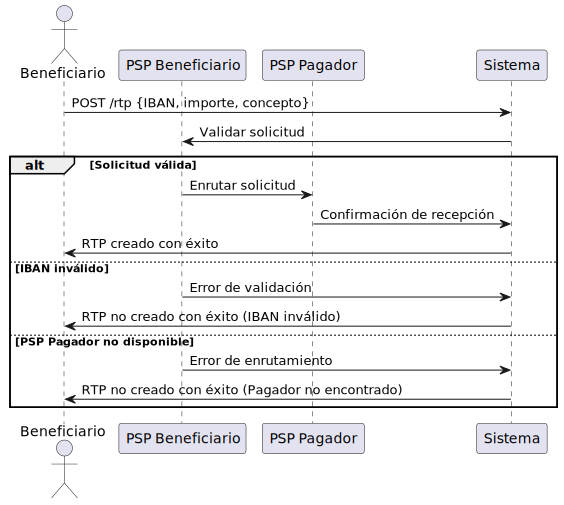
\includegraphics[width=.9\textwidth]{Imagenes/CU01.pdf}
  \caption{Diagrama de secuencia para CU‑01 (crear solicitud RTP).}
  \label{fig:seq_cu01}
\end{figure}

\begin{figure}[htbp]
  \centering
  % placeholder
  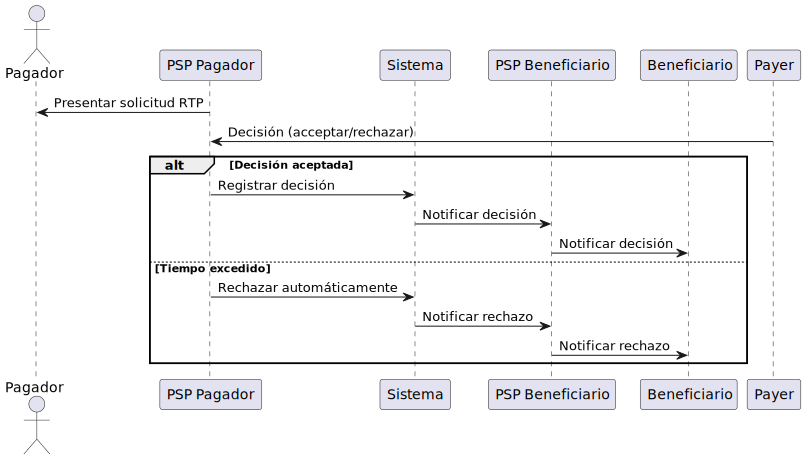
\includegraphics[width=.9\textwidth]{Imagenes/CU02.pdf}
  \caption{Diagrama de secuencia para CU‑02 (decisión final RTP).}
  \label{fig:seq_cu02}
\end{figure}

\section{Modelo de datos}
\label{subsec:diseno_datos}

% Descripción del esquema de la base de datos y referencia a la figura del modelo ER
El esquema de la base de datos, representado en el modelo entidad-relación (ER) de la Figura~\ref{fig:er_model}, está diseñado para soportar el flujo del esquema SRTP. Consta de tres tablas principales: \texttt{Actor}, \texttt{RTP} y \texttt{Log}, cada una con atributos específicos para almacenar la información necesaria del sistema.

% Inclusión de la figura del modelo ER
\begin{figure}[htbp]
  \centering
  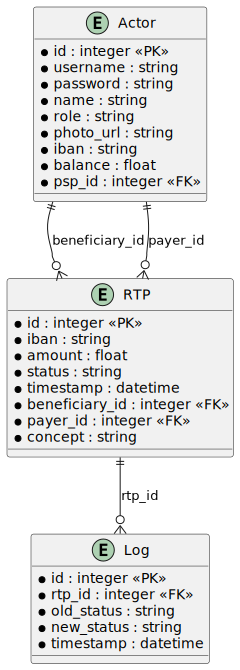
\includegraphics[width=0.9\textwidth, height=0.9\textheight, keepaspectratio]{Imagenes/ER.pdf}
  \caption{Modelo entidad-relación del prototipo.}
  \label{fig:er_model}
\end{figure}

% Listado de las tablas y sus atributos
Las tablas que componen el modelo de datos son las siguientes:

\begin{itemize}
  \item \textbf{Actor} (\texttt{id}, \texttt{username}, \texttt{password}, \texttt{name}, \texttt{role}, \texttt{photo\_url}, \texttt{iban}, \texttt{balance}, \texttt{psp\_id}) --- Almacena información sobre los actores involucrados en el sistema, como beneficiarios, pagadores y proveedores de servicios de pago (PSP). Sus atributos son:
    \begin{itemize}
      \item \texttt{id}: Identificador único del actor (clave primaria).
      \item \texttt{username}: Nombre de usuario único para autenticación.
      \item \texttt{password}: Contraseña del actor.
      \item \texttt{name}: Nombre completo del actor.
      \item \texttt{role}: Rol del actor, que puede ser \emph{beneficiary}, \emph{psp\_beneficiary}, \emph{psp\_payer} o \emph{payer}.
      \item \texttt{photo\_url}: URL o base64 de la foto del actor (opcional).
      \item \texttt{iban}: Número de cuenta bancaria internacional (IBAN).
      \item \texttt{balance}: Saldo disponible del actor.
      \item \texttt{psp\_id}: Referencia al actor que actúa como PSP (clave foránea a \texttt{Actor}).
    \end{itemize}

  \item \textbf{RTP} (\texttt{id}, \texttt{iban}, \texttt{amount}, \texttt{status}, \texttt{timestamp}, \texttt{beneficiary\_id}, \texttt{psp\_beneficiary\_id}, \texttt{psp\_payer\_id}, \texttt{payer\_id}, \texttt{concept}) --- Registra las solicitudes de pago (\emph{Request To Pay}). Sus atributos son:
    \begin{itemize}
      \item \texttt{id}: Identificador único de la solicitud (clave primaria).
      \item \texttt{iban}: IBAN del pagador.
      \item \texttt{amount}: Monto de la solicitud de pago.
      \item \texttt{status}: Estado actual de la solicitud (e.g., "creado").
      \item \texttt{timestamp}: Fecha y hora de creación de la solicitud.
      \item \texttt{beneficiary\_id}: Referencia al actor beneficiario.
      \item \texttt{psp\_beneficiary\_id}: Referencia al PSP del beneficiario.
      \item \texttt{psp\_payer\_id}: Referencia al PSP del pagador.
      \item \texttt{payer\_id}: Referencia al actor pagador.
      \item \texttt{concept}: Descripción o motivo de la solicitud de pago.
    \end{itemize}

  \item \textbf{Log} (\texttt{id}, \texttt{rtp\_id}, \texttt{old\_status}, \texttt{new\_status}, \texttt{timestamp}, \texttt{hash\_value}) --- Almacena el historial de cambios de estado de las solicitudes RTP. Sus atributos son:
    \begin{itemize}
      \item \texttt{id}: Identificador único del registro (clave primaria).
      \item \texttt{rtp\_id}: Referencia a la solicitud RTP asociada.
      \item \texttt{old\_status}: Estado anterior de la solicitud.
      \item \texttt{new\_status}: Nuevo estado de la solicitud.
      \item \texttt{timestamp}: Marca de tiempo del cambio de estado.
      \item \texttt{hash\_value}: Hash para verificar la integridad del registro.
    \end{itemize}
\end{itemize}

% Explicación del mecanismo de hash y las relaciones entre tablas
El atributo \texttt{hash\_value} de la tabla \texttt{Log} se calcula utilizando el algoritmo SHA-256 sobre una concatenación de campos clave, como \texttt{rtp\_id}, \texttt{old\_status}, \texttt{new\_status} y \texttt{timestamp}. Este hash asegura la integridad de cada entrada, permitiendo detectar cualquier modificación no autorizada en el historial de estados.

Las relaciones entre las tablas están definidas mediante claves foráneas:
- En \texttt{RTP}, los campos \texttt{beneficiary\_id}, \texttt{psp\_beneficiary\_id}, \texttt{psp\_payer\_id} y \texttt{payer\_id} referencian a \texttt{Actor.id}.
- En \texttt{Log}, \texttt{rtp\_id} referencia a \texttt{RTP.id}.
- En \texttt{Actor}, \texttt{psp\_id} referencia a otro \texttt{Actor.id}, estableciendo una relación recursiva para indicar el PSP asociado.

Todas las claves foráneas están configuradas con \emph{\texttt{ON DELETE CASCADE}}, lo que significa que la eliminación de un registro en una tabla padre (como \texttt{Actor} o \texttt{RTP}) provocará la eliminación automática de los registros dependientes en las tablas hijas (como \texttt{RTP} o \texttt{Log}), facilitando las pruebas y el mantenimiento del prototipo.


\section{Arquitectura lógica}
\label{subsec:diseno_arquitectura}

La arquitectura lógica del prototipo, ilustrada en la Figura~\ref{fig:componentes}, organiza los componentes del sistema en capas para garantizar una separación clara de responsabilidades y facilitar la escalabilidad y el mantenimiento. El diseño se basa en un enfoque modular que permite simular el flujo del esquema SRTP en un entorno distribuido, utilizando tecnologías modernas como REST y WebSocket para la comunicación y SQLAlchemy para la persistencia.

% Inclusión de la figura de la arquitectura
\begin{figure}[htbp]
  \centering
  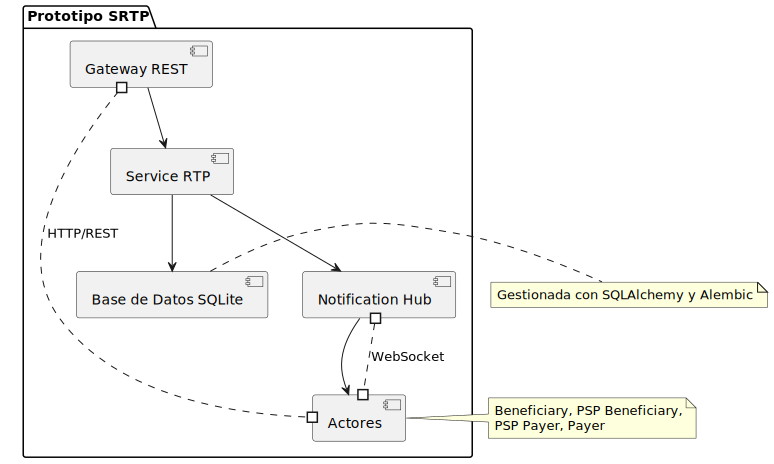
\includegraphics[width=.85\textwidth]{Imagenes/DiagComp.pdf}
  \caption{Arquitectura lógica y flujo de dependencias del prototipo.}
  \label{fig:componentes}
\end{figure}

% Descripción de los componentes principales
\subsection{Componentes principales}
\label{subsec:componentes_principales}
El sistema se estructura en tres componentes principales:
\begin{itemize}
  \item \textbf{Gateway REST}: Actúa como punto de entrada para las solicitudes HTTP, gestionando la validación inicial de las peticiones y enrutándolas al componente adecuado. Este componente asegura que las solicitudes cumplan con los formatos esperados antes de procesarlas.
  \item \textbf{Service RTP}: Encapsula la lógica de negocio del esquema SRTP, incluyendo la creación, validación, enrutamiento y decisión de solicitudes de pago. Interactúa con la base de datos para almacenar y recuperar información.
  \item \textbf{Notification Hub}: Mantiene canales WebSocket abiertos con los cuatro actores del modelo de cuatro esquinas (Beneficiary, PSP Beneficiary, PSP Payer y Payer), enviando notificaciones en tiempo real sobre eventos como la creación o decisión de una solicitud RTP.
\end{itemize}

%----------------------------------------------
% 3.6.2 – Flujo de interacción lógico
%----------------------------------------------
\subsection{Flujo de interacción lógico}
\label{subsec:flujo_interaccion}

El ciclo \textbf{SRTP} se articula en los cuatro pasos lógicos que se detallan a continuación:

\begin{enumerate}[label=\arabic*.]
  \item \textbf{Recepción} – El \emph{Gateway} recibe la petición
        \verb|POST /rtp| y la delega al \emph{Service RTP}.
  \item \textbf{Procesamiento} – El \emph{Service RTP} aplica la lógica de negocio
        y actualiza el estado
        \mbox{\texttt{created} $\rightarrow$ \texttt{validated} $\rightarrow$ \texttt{routed} …}.
  \item \textbf{Publicación} – Tras cada transición de estado válida,
        el servicio emite un evento de dominio.
  \item \textbf{Notificación} – El \emph{Notification Hub} reenvía dicho evento,
        vía WebSocket, a las salas correspondientes
        (\emph{psp\_beneficiary}, \emph{psp\_payer}, \emph{payer} o \emph{beneficiary}).
\end{enumerate}

Con este patrón se obtienen las siguientes ventajas:

\begin{itemize}
  \item Los \emph{clientes} no interrogan al servidor; reciben notificaciones \emph{push}.
  \item La \emph{consistencia} del estado queda centralizada en el \emph{Service RTP}.
  \item El sistema puede escalar horizontalmente añadiendo réplicas del servicio
        sin romper el contrato público.
\end{itemize}



\section{Emulación del flujo RTP}
\label{subsec:emulacion_flujo_rtp}

% Inclusión de la figura de la máquina de estados
\begin{figure}[htbp]
  \centering
  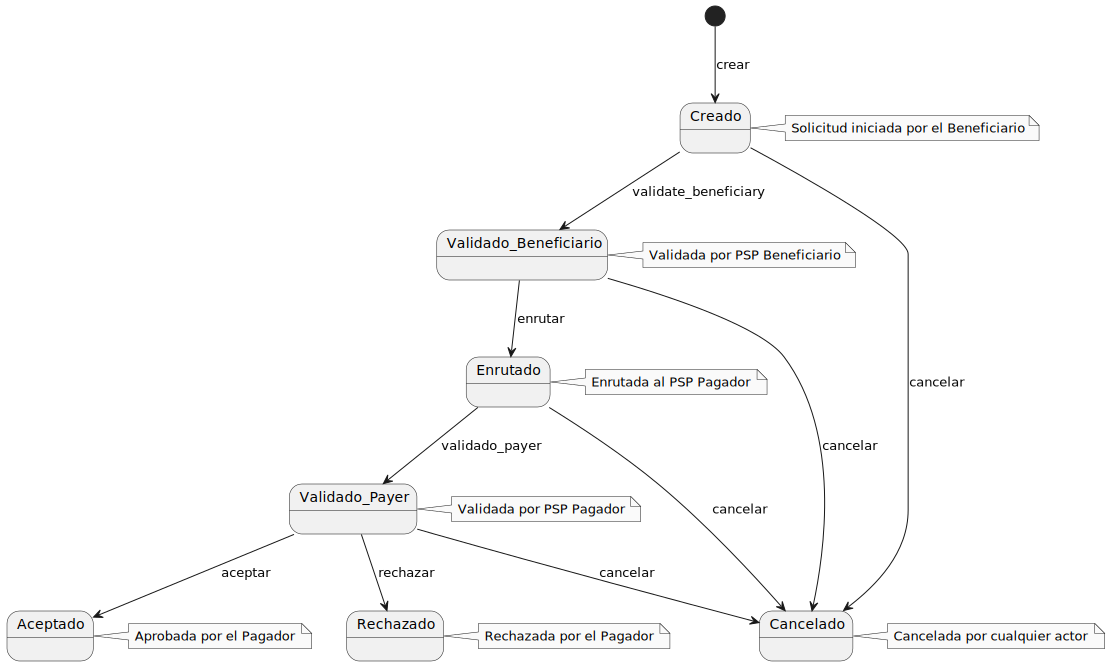
\includegraphics[width=.85\textwidth]{Imagenes/DiagEstado.pdf}
  \caption{Máquina de estados del objeto RTP.}
  \label{fig:state_machine_rtp}
\end{figure}

El objetivo de este apartado es describir cómo el prototipo recrea, de extremo a extremo, el ciclo de vida de una solicitud RTP dentro del bloque \textbf{Service RTP}, único responsable de aplicar la lógica de negocio y salvaguardar la coherencia del estado global. A diferencia de otros componentes, este servicio actúa como \emph{single source of truth}: valida, persiste, publica eventos de dominio y rechaza cualquier transición inválida.

\subsection{Máquina de estados del objeto RTP}
\label{subsec:rtp_state_machine}

La Figura~\ref{fig:state_machine_rtp} sintetiza el recorrido que puede seguir una solicitud:  
\textbf{Creado $\rightarrow$ Validado Beneficiario $\rightarrow$ Enrutado $\rightarrow$ Validado Payer $\rightarrow$ (Aceptado $|$ Rechazado $|$ Cancelado)}.  
Cada arista representa una operación expuesta por la API (por ejemplo, \texttt{create}, \texttt{validate\_beneficiary}, \texttt{route}, \texttt{validate\_payer}, \texttt{accept}, \texttt{reject}, \texttt{cancel}) y sólo puede ejecutarse si el objeto se encuentra en el estado de origen indicado.

\subsection{Transiciones y reglas de negocio}

\begin{description}
  \item[\textbf{Creación} (\texttt{create})]  
        El \emph{Beneficiary} emite un \texttt{POST /rtp}. \textbf{Service RTP} valida sintaxis y semántica (IBAN, ISO 4217, etc.), calcula un hash SHA-256 para evitar duplicados y persiste el registro como \textsc{CREADO}.
  \item[\textbf{Validación del PSP Beneficiary} (\texttt{validate\_beneficiary})]  
        El PSP del beneficiario comprueba el cumplimiento de las reglas SRTP (formato, AML/KYC básico). Si falla, genera un \texttt{reject} inmediato con motivo normalizado.
  \item[\textbf{Enrutado} (\texttt{route})]  
        Una vez validada, la solicitud se envía al PSP \emph{Payer}. El estado avanza a \textsc{ENRUTADO} y se incorpora un \texttt{timestamp} a la traza.
  \item[\textbf{Validación del PSP Payer} (\texttt{validate\_payer})]  
        El PSP del pagador confirma que el cliente puede recibir la solicitud. La aprobación conduce a \textsc{VALIDADO\_PAYER}; de lo contrario, devuelve \texttt{reject}.
  \item[\textbf{Decisión del Payer} (\texttt{accept} / \texttt{reject})]  
        El pagador dispone de un máximo de diez segundos para responder. La aceptación transita a \textsc{ACEPTADO}; la denegación, a \textsc{RECHAZADO}.
  \item[\textbf{Cancelación} (\texttt{cancel})]  
        Cualquiera de los cuatro actores puede solicitar la anulación antes de la decisión final, llevando el flujo a \textsc{CANCELADO}.
\end{description}

Todas las reglas están encapsuladas en métodos de dominio homogéneos en firma y manejo de errores, favoreciendo la mantenibilidad y la trazabilidad entre diseño y código.

\subsection{Condiciones excepcionales y \emph{timeouts}}

Si el pagador no responde antes de la \textbf{fecha/hora de expiración} definida en la solicitud, el sistema ejecuta una transición automática a \textsc{CANCELADO}. Del mismo modo, cualquier error técnico de un PSP desemboca en un \texttt{reject}, manteniendo la consistencia global sin intervención manual.
%
%\subsection{Resumen}
%
%El modelo de estados implementado consagra tres principios:
%
%\begin{enumerate}
%  \item \textbf{Centralización}: toda la lógica reside en \textbf{Service RTP}, evitando duplicidades y condiciones de carrera.
%  \item \textbf{Observabilidad}: cada evento se persiste, firma y publica, facilitando auditoría y \emph{monitoring}.
%  \item \textbf{Extensibilidad}: la adición de nuevos estados o transiciones (p.\,ej.\ \emph{refund}) sólo requiere ampliar la máquina y los servicios asociados, sin impactar capas externas.
%\end{enumerate}
%
%
%Con ello, la emulación demuestra que el ciclo SRTP puede implementarse de forma robusta y trazable aprovechando patrones de \emph{domain-driven design} y mensajería asíncrona, sentando las bases para una futura conexión con infraestructuras de pago reales.

\newpage



% 3. Diseño e Implementación
\input{src/implementacion.tex}
%\newpage
\newpage



\input{src/validacion.tex}
\newpage



\newpage
\chapter{Conclusiones}
\label{sec:Conclusiones}

El desarrollo de este TFG ha representado un esfuerzo significativo que ha culminado en la creación de un prototipo funcional de un servidor HTTP basado en el esquema RTP. El objetivo principal del proyecto —diseñar e implementar un software que simulara las operaciones fundamentales del esquema SEPA RTP utilizando tecnologías actuales y accesibles— se ha alcanzado con éxito. Este trabajo no solo me ha permitido poner en práctica los conocimientos adquiridos durante mi formación en telecomunicaciones y desarrollo de software, sino también explorar un ámbito tan relevante como los sistemas de pago digitales, que desempeñan un papel crucial en la economía global de hoy.

\vspace{0.5cm}

A nivel personal, este TFG ha sido una buena oportunidad para profundizar en el ecosistema SEPA y sus diferentes esquemas de pago. En particular, he podido analizar las limitaciones del SDD y contrastarlas con las ventajas que ofrece RTP. Este aprendizaje no se ha limitado al ámbito teórico: la implementación práctica del prototipo me ha enfrentado a retos técnicos que han fortalecido mis competencias como desarrollador.

\vspace{0.5cm}

El proceso de desarrollo también ha sido una lección sobre la importancia de una metodología bien definida, lo que me permitió avanzar de manera constante, detectar errores a tiempo y ajustar los objetivos según las necesidades del proyecto. Este enfoque estructurado, combinado con una documentación detallada de cada etapa, ha sido clave para mantener el control sobre el proyecto.
\vspace{0.5cm}


El sistema RTP se posiciona como un candidato ideal paraq convertirse en un estándar en la zona SEPA, especialmente a medida que más instituciones financieras y PSP adopten el esquema y lo integren en sus operaciones. En el futuro, es probable que RTP no solo facilite los pagos entre empresas y consumidores, sino que también fomente una mayor interoprabilidad y eficiencia en el mercado financiaro europeo, contribuyendo a una economía más conectada y dinámica.
\vspace{0.5cm}

\newpage
\null
\clearpage
\chapter{Líneas futuras}
\label{sec:Potencial}
En cuanto al prototipo desarollado, aunque satisface plenamente los objetivos establecidos para este TFG, su potencial va mucho más allá de un simple ejercicio acádemico. Durante el proceso identifiqué varias áreas de mejora que podrían transformar este simulador en una herramienta aplicable en escenarios reales. A continuación, detallo algunas de estas oportunidades de evolución:

\begin{enumerate}
    \item \textbf{Escalabilidad del sistema:} La base de datos SQLite, aunque suficiente para un prototipo, tiene limitaciones en térmninos de rendimiento y capacidad. Para soportar un mayor volumen de usuarios y transacciones, sería necesario migrar a un sistema más robusto como PostgreSQL o MySQL, que ofrecen mejor escalabilidad y soporte para entornos de producción.
    \item \textbf{Fortalecimiento de la seguridad:} El prototipo incluye medidas básicas de autenticación, pero un sistema real requeriría estándares más altos, como la encriptación de extremo a extremo, autenticación multifactor y cumplimiento con normativas como PSD2 (Payment Services Directive 2) y GDPR (General Data Protection Regulation). Estas mejoras garantizarían la protección de los datos sensibles y la confianza de los usuarios.
    \item \textbf{Interoperabilidad con sistemas bancarios:} Para que el prototipo trascienda su estado actual, sería esencial integrarlo con las APIs de bancos y PSP reales. Esto permitiría ejecutar transacciones monetarias auténticas y demostrar su utilidad en un contexto práctico, un paso crítico hacia su adopción en el mundo real.
    \item \textbf{Ampliación de funcionalidades:} El sistema podría enriquecerse con características avanzadas, como soporte para pagos recurrentes (ideal para suscripciones o facturas periódicas), compatibilidad con múltiples monedas (facilitando transacciones transfronterizas), herramientas analíticas que ofrezcan estadísticas a los usuarios, y reportes detallados sobre el historial de pagos. Estas adiciones harían que el sistema fuera más versátil y atractivo para distintos tipos de usuarios.
    \item \textbf{Mejora de la experiencia de usario:} Aunque el frontend actual es funcional, podría optimizarse con un diseño más moderno y accesible. Incorporar elementos como notificaciones push, un historial visual de transacciones, opciones de personalización y una interfaz adaptada a dispositivos móviles elevaría la usabilidad y la satisfacción del usuario.
\end{enumerate}

Estas mejoras, aunque son algo ambiciosas, son alcanzables con el tiempo y los recursos adecuados. Implementarlas no solo incrementaría la funcionalidad del prototipo, sino que también lo alinearía con las demandas de un mercado financiero en constante camnbio, donde la innovación y la adaptabilidad son esenciales.
\vspace{0.5cm}
\newpage
% Añadiendo los apéndices
\clearpage




\newpage

\backmatter

\lstinputlisting[language=Python, style=custom, caption={RF-01 Crear Solicitud RTP services.py}, label={lst:1}, firstline=6, lastline=52]{../backend/services.py}
\lstinputlisting[language=Python, style=custom, caption={RF-01 Crear Solicitud RTP routes.py}, label={lst:2}, firstline=14, lastline=37]{../backend/routes.py}
\lstinputlisting[language=Python, style=custom, caption={RF-01 Crear Solicitud RTP RTP.js}, label={lst:3}, firstline=40, lastline=71]{../frontend/RTP.js}

\lstinputlisting[language=Python, style=custom, caption={RF-02 Validar y enrutar RTP services.py}, label={lst:4}, firstline=53, lastline=74]{../backend/services.py}
\lstinputlisting[language=Python, style=custom, caption={RF-02 Validar y enrutar RTP routes.py}, label={lst:5}, firstline=37, lastline=53]{../backend/routes.py}
\lstinputlisting[language=Python, style=custom, caption={RF-02 Validar y enrutar RTP utils.py}, label={lst:6}, firstline=30, lastline=70]{../backend/utils.py}
\lstinputlisting[language=Python, style=custom, caption={RF-02 Validar y enrutar RTP RTP.js}, label={lst:7}, firstline=71, lastline=117]{../frontend/RTP.js}

\lstinputlisting[language=Python, style=custom, caption={RF-03 Validación pagador services.py}, label={lst:8}, firstline=74, lastline=102]{../backend/services.py}
\lstinputlisting[language=Python, style=custom, caption={RF-03 Validación pagador routes.py}, label={lst:9}, firstline=54, lastline=61]{../backend/routes.py}
\lstinputlisting[language=Python, style=custom, caption={RF-03 Validación pagador RTP.js}, label={lst:10}, firstline=117, lastline=140]{../frontend/RTP.js}

\lstinputlisting[language=Python, style=custom, caption={RF-04 Decisión final services.py}, label={lst:11}, firstline=103, lastline=137]{../backend/services.py}
\lstinputlisting[language=Python, style=custom, caption={RF-04 Decisión final routes.py}, label={lst:12}, firstline=62, lastline=70]{../backend/routes.py}
\lstinputlisting[language=Python, style=custom, caption={RF-04 Decisión final RTP.js}, label={lst:13}, firstline=141, lastline=167]{../frontend/RTP.js}



\begin{lstlisting}[language=Python, style=custom, caption={RF-05 Notificación ext\_socketio.py}, label={lst:14}]
    # ext_socketio.py
    from flask_socketio import SocketIO, join_room, emit

    socketio = SocketIO()
\end{lstlisting}


\lstinputlisting[language=Python, style=custom, caption={RF-05 Notificación services.py}, label={lst:15}, firstline=131, lastline=134]{../backend/services.py}
\lstinputlisting[language=Python, style=custom, caption={RF-05 Notificación RTP.js}, label={lst:16}, firstline=333, lastline=362]{../frontend/RTP.js}

%AQUI IRÍA RF-06

%RNF-01 no codigo necesario

%RNF-02 Depende de dockerfile

\lstinputlisting[language=Python, style=custom, caption={RNF-02 Seguridad y trazabilidad utils.py}, label={lst:17}, firstline=3, lastline=25]{../backend/utils.py}
\lstinputlisting[language=Python, style=custom, caption={RNF-02 Seguridad y trazabilidad models.py}, label={lst:18}, firstline=58, lastline=77]{../backend/models.py}

\lstinputlisting[language=Python, style=custom, caption={RNF-03 Portabilidad  config.py}, label={lst:19}, firstline=1, lastline=8]{../backend/config.py}
\lstinputlisting[language=Python, style=custom, caption={RNF-03 Portabilidad  requirements.txt}, label={lst:20}, firstline=1, lastline=3]{../backend/requirements.txt}
\lstinputlisting[language=Python, style=custom, caption={RNF-03 Portabilidad  app.py}, label={lst:21}, firstline=1, lastline=55]{../backend/app.py}

%RNF-05


\lstinputlisting[language=Python, style=custom, caption={clase Actor}, label={lst:22}, firstline=5, lastline=32]{../backend/models.py}
\lstinputlisting[language=Python, style=custom, caption={clase RTP}, label={lst:23}, firstline=34, lastline=57]{../backend/models.py}
\lstinputlisting[language=Python, style=custom, caption={clase Log}, label={lst:24}, firstline=59, lastline=76]{../backend/models.py}


% Añadiendo el índice de figuras
\newpage
\renewcommand{\listfigurename}{Índice de Figuras}
\listoffigures
\addcontentsline{toc}{section}{Índice de Figuras}

% Añadiendo el índice de tablas
\newpage
\renewcommand{\listtablename}{Índice de Tablas}
\listoftables
\addcontentsline{toc}{section}{Índice de Tablas}

% Añadiendo el índice de códigos
\newpage
\renewcommand*{\lstlistlistingname}{Índice de Listados}
\renewcommand*{\lstlistingname}{Código}
\lstlistoflistings
\addcontentsline{toc}{section}{Índice de Listados}

% Añadiendo las referencias
\clearpage
\nocite{*}
\printbibliography[title={Bibliografía}]


\end{document}